%%%%%% Run at command line, run
%%%%%% xelatex grad-sample.tex 
%%%%%% for a few times to generate the output pdf file
\documentclass[12pt,oneside,openright,a4paper]{cpe-english-project}

\usepackage{polyglossia}
\usepackage{tabularx}
%\usepackage{algorithm}
\setdefaultlanguage{english}
\setotherlanguage{thai}
\newfontfamily\thaifont[Script=Thai,Scale=1.23]{TH Sarabun New}
\defaultfontfeatures{Mapping=tex-text,Scale=1.0,LetterSpace=0.0}
\setmainfont[Scale=1.0,LetterSpace=0,WordSpace=1.0,FakeStretch=1.0]{Times New Roman}

% Custom setting
\setlength{\parskip}{1em} % Set paragraph margin
% Set nested numuric list
\renewcommand{\labelenumii}{\theenumii}
\renewcommand{\theenumii}{\theenumi.\arabic{enumii}.}
\renewcommand{\labelenumiii}{\theenumiii}
\renewcommand{\theenumiii}{\theenumii.\arabic{enumiii}.}
% End set nested numuric list

%\setmathfont(Digits)[Scale=1.0,LetterSpace=0,FakeStretch=1.0]{Times New Roman}


%%%%%%%%%%%%%%%%%%%%%%%%%%%%%%%%%%%%%%%%%%%%%%%%%%%%%%%%%%%%%%%%%%%
% Customize below to suit your needs 
% The ones that are optional can be left blank. 
%%%%%%%%%%%%%%%%%%%%%%%%%%%%%%%%%%%%%%%%%%%%%%%%%%%%%%%%%%%%%%%%%%%
% First line of title
\def\disstitleone{PROJECT NO. 72}   
% Second line of title
\def\disstitletwo{A RESTAURANT RECOMMENDATION SYSTEM FOR INDIVIDUALS AND GROUPS}   
% Your first name and lastname
\def\dissauthor{MR. CHANCHANA WICHA}   % 1st member
\def\dissauthortwo{MS. IRIN YOOKTAJARONG}   % 2nd member (optional)
\def\dissauthorthree{}


% The degree that you're persuing..
\def\dissdegree{Bachelor of Engineering} % Name of the degree
\def\dissdegreeabrev{B.Eng} % Abbreviation of the degree
\def\dissyear{2020}                   % Year of submission
\def\thaidissyear{2563}               % Year of submission (B.E.)

%%%%%%%%%%%%%%%%%%%%%%%%%%%%%%%%%%%%%%%%%%%%
% Your project and independent study committee..
%%%%%%%%%%%%%%%%%%%%%%%%%%%%%%%%%%%%%%%%%%%%
\def\dissadvisor{Dr. Unchalisa Taetragool, Ph.D.}  % Advisor
%%% Leave it empty if you have no Co-advisor
\def\disscoadvisor{}  % Co-advisor
\def\disscommitteetwo{Asst.Prof.Dr. Rajchawit Sarochawikasit, Ph.D.}  % 3rd committee member (optional)
\def\disscommitteethree{Dr. Sally E. Goldin, Ph.D.}   % 4th committee member (optional) 
\def\disscommitteefour{Asst.Prof.Mr. Sanan Srakaew, B.Eng.}    % 5th committee member (optional) 

\def\worktype{Project} %%  Project or Independent study
\def\disscredit{3}   %% 3 credits or 6 credits


\def\fieldofstudy{Computer Engineering} 
\def\department{Computer Engineering} 
\def\faculty{Engineering}

\def\thaifieldofstudy{วิศวกรรมคอมพิวเตอร์} 
\def\thaidepartment{วิศวกรรมคอมพิวเตอร์} 
\def\thaifaculty{วิศวกรรมศาสตร์}
 
\def\appendixnames{Appendix} %%% Appendices or Appendix

\def\thaiworktype{ปริญญานิพนธ์} %  Project or research project % 
\def\thaidisstitleone{หัวข้อปริญญานิพนธ์บรรทัดแรก}
\def\thaidisstitletwo{หัวข้อปริญญานิพนธ์บรรทัดสอง}
\def\thaidissauthor{นายชาญชนะ วิชา}
\def\thaidissauthortwo{นางสาวไอริณ ยุกตจรงค์} %Optional
\def\thaidissauthorthree{} %Optional

\def\thaidissadvisor{ดร. อัญชลิสา แต้ตระกูล}
%% Leave this empty if you have no co-advisor
\def\thaidisscoadvisor{} %Optional
\def\thaidissdegree{วิศวกรรมศาสตรบัณฑิต}

% Change the line spacing here...
\linespread{1.15}

%%%%%%%%%%%%%%%%%%%%%%%%%%%%%%%%%%%%%%%%%%%%%%%%%%%%%%%%%%%%%%%%
% End of personal customization.  Do not modify from this part 
% to \begin{document} unless you know what you are doing...
%%%%%%%%%%%%%%%%%%%%%%%%%%%%%%%%%%%%%%%%%%%%%%%%%%%%%%%%%%%%%%%%


%%%%%%%%%%%% Dissertation style %%%%%%%%%%%
%\linespread{1.6} % Double-spaced  
%%\oddsidemargin    0.5in
%%\evensidemargin   0.5in
%%%%%%%%%%%%%%%%%%%%%%%%%%%%%%%%%%%%%%%%%%%
%\renewcommand{\subfigtopskip}{10pt}
%\renewcommand{\subfigbottomskip}{-5pt} 
%\renewcommand{\subfigcapskip}{-6pt} %vertical space between caption
%                                    %and figure.
%\renewcommand{\subfigcapmargin}{0pt}

\renewcommand{\topfraction}{0.85}
\renewcommand{\textfraction}{0.1}

\newtheorem{theorem}{Theorem}
\newtheorem{lemma}{Lemma}
\newtheorem{corollary}{Corollary}

\def\QED{\mbox{\rule[0pt]{1.5ex}{1.5ex}}}
\def\proof{\noindent\hspace{2em}{\itshape Proof: }}
\def\endproof{\hspace*{\fill}~\QED\par\endtrivlist\unskip}
%\newenvironment{proof}{{\sc Proof:}}{~\hfill \blacksquare}
%% The hyperref package redefines the \appendix. This one 
%% is from the dissertation.cls
%\def\appendix#1{\iffirstappendix \appendixcover \firstappendixfalse \fi \chapter{#1}}
%\renewcommand{\arraystretch}{0.8}
%%%%%%%%%%%%%%%%%%%%%%%%%%%%%%%%%%%%%%%%%%%%%%%%%%%%%%%%%%%%%%%%
%%%%%%%%%%%%%%%%%%%%%%%%%%%%%%%%%%%%%%%%%%%%%%%%%%%%%%%%%%%%%%%%


\begin{document}
\pdfstringdefDisableCommands{%
\let\MakeUppercase\relax
}
\begin{center}
  
\includegraphics[width=2.8cm]{logo02.jpg}
\end{center}
\vspace*{-1cm}

\maketitlepage
\makesignaturepage 

%%%%%%%%%%%%%%%%%%%%%%%%%%%%%%%%%%%%%%%%%%%%%%%%%%%%%%%%%%%%%%
%%%%%%%%%%%%%%%%%%%%%% English abstract %%%%%%%%%%%%%%%%%%%%%%%
%%%%%%%%%%%%%%%%%%%%%%%%%%%%%%%%%%%%%%%%%%%%%%%%%%%%%%%%%%%%%%
\abstract

In recent years, recommendation systems are widely used for movies, music, or products in order to reduce the time and effort of the users’ searching and increase users’ experience. However, restaurant recommendation systems are still very few in this industry and the existing recommenders in Thailand are just randomization applications and the majority of recommender systems are designed for individual users. In contrast, since this activity or event usually occurs in a group of people, not just individually, which each person can have the same or different behaviors, preferences, and interests. Therefore, group decisions often differ from individual decisions. As a result, each decision is often taken longer than one person, and sometimes conclusions are not able to be drawn or it may cause conflicts within the group.

According to the mentioned problems, we were motivated to develop this project, A Restaurant Recommendation System for Individuals and Groups, to better assist in group decision making. Our project is a web application that recommends restaurants in the Bangkok area to users based on their behaviors, preferences, and interests of both individuals and groups eating. The genetic algorithm is applied for generating suitable recommended restaurants for users. Therefore, this project aims to reduce time-wasting of decision making for both individuals and groups and increase the users’ experience and satisfaction when using our recommendation system.


\begin{flushleft}
\begin{tabular*}{\textwidth}{@{}lp{0.8\textwidth}}
\textbf{Keywords}: & Genetic Algorithm / Optimization Problem / Decision Making Process / Group Recommendation Systems / Web Application / Restaurants
\end{tabular*}
\end{flushleft}
\endabstract

%%%%%%%%%%%%%%%%%%%%%%%%%%%%%%%%%%%%%%%%%%%%%%%%%%%%%%%%%%%%%%
%%%%%%%%%% Thai abstract here %%%%%%%%%%%%%%%%%%%%%%%%%%%%%%%%%
%%%%%%%%%%%%%%%%%%%%%%%%%%%%%%%%%%%%%%%%%%%%%%%%%%%%%%%%%%%%%%
{
\XeTeXlinebreaklocale "th_TH"	
\thaifont
\thaiabstract

ในช่วงไม่กี่ปีที่ผ่านมาได้มีการใช้ระบบแนะนำ (Recommendation System) อย่างแพร่หลายไม่ว่าจะเป็นภาพยนตร์ เพลง หรือระบบแนะนำผลิตภัณฑ์ต่าง ๆ เพื่อลดระยะเวลาและความยุ่งยากในการค้นหาของผู้ใช้รวมถึงเพิ่มประสบการณ์ของผู้ใช้อย่างไรก็ตามระบบแนะนำร้านอาหารยังมีน้อยมากในวงการระบบคำแนะนำนอกจากนั้นระบบแนะนำร้านอาหารที่มีอยู่ในประเทศไทยเป็นเพียงแอปพลิเคชันแบบสุ่มและส่วนใหญ่ออกแบบมาสำหรับผู้ใช้แต่ละรายเท่านั้น ซึ่งในความเป็นจริงแล้วการรับประทานอาหารมักเกิดขึ้นเป็นกลุ่มตั้งแต่ 2 คนขึ้นไปไม่ได้เป็นรายบุคคลเพียงอย่างเดียว ซึ่งแต่ละคนในกลุ่มนั้นมีพฤติกรรม ความชอบและความสนใจที่อาจจะเหมือนหรือแตกต่างกันดังนั้นการตัดสินใจของกลุ่มมักแตกต่างจากการตัดสินใจของแต่ละบุคคล ด้วยเหตุนี้การตัดสินใจในแต่ละครั้ง มักใช้เวลานานกว่าการตัดสินใจด้วยคน ๆ เดียว และในบางครั้งการตัดสินใจนั้นอาจจะไม่สามารถหาข้อสรุปได้ หรืออาจทําให้เกิดความขัดแย้งขึ้นภายในกลุ่ม

ด้วยเหตุนี้เอง ทางผู้พัฒนาจึงมีความตั้งใจที่จะพัฒนาเว็บแอปพลิเคชันสำหรับแนะนำร้านอาหารที่อยู่ในพื้นที่จังหวัดกรุงเทพมหานครสำหรับรายบุคคลและรายกลุ่มขึ้น เพื่อเป็นตัวช่วยในการตัดสินใจทั้งแบบเดี่ยวและกลุ่มได้ดีมากยิ่งขึ้น โดยระบบแนะนําร้านอาหารจะอ้างอิงจากข้อมูลของผู้ใช้งาน ไม่ว่าจะเป็นพฤติกรรม ความสนใจ หรือความชอบ ทั้งแบบเดี่ยวและกลุ่ม ด้วยขั้นตอนวิธีเชิงพันธุกรรม (Genetic Algorithm) ในการหาค่าเหมาะสมที่สุดเชิงคณิตศาสตร์ (Mathematical Optimization) สุดท้ายนี้ผู้พัฒนามีความมุ่งหวังว่าระบบแนะนําร้านอาหารรายบุคคลและรายกลุ่มในโครงงานนี้จะช่วยลดเวลาที่เสียไปในการตัดสินใจและเพิ่มความพึงพอใจของผู้ใช้งานต่อร้านอาหารที่ระบบได้ทำการแนะนำ


\begin{flushleft}
\begin{tabular*}{\textwidth}{@{}lp{0.8\textwidth}}
 & \\

\textbf{คำสำคัญ}: & ขั้นตอนวิธีเชิงพันธุกรรม / การหาค่าเหมาะสมที่สุดเชิงคณิตศาสตร์ / กระบวนการการตัดสินใจ / ระบบแนะนำรายกลุ่ม / เว็บแอปพลิเคชัน / ร้านอาหาร
\end{tabular*}
\end{flushleft}
\endabstract
}

%%%%%%%%%%%%%%%%%%%%%%%%%%%%%%%%%%%%%%%%%%%%%%%%%%%%%%%%%%%%
%%%%%%%%%%%%%%%%%%%%%%% Acknowledgments %%%%%%%%%%%%%%%%%%%%
%%%%%%%%%%%%%%%%%%%%%%%%%%%%%%%%%%%%%%%%%%%%%%%%%%%%%%%%%%%%
\preface
Throughout the writing of this project we have received a great deal of support and assistance.

We would like to express my very great appreciation to Dr. Unchalisa Taetragool for her valuable and constructive suggestions during the planning and development of this project work. Her willingness to give his time so generously has been very much appreciated.

We would also like to express our very great appreciation to our committees, Asst.Prof.Dr. Rajchawit Sarochawikasit, Dr. Sally E. Goldin and Asst.Prof.Mr. Sanan Srakaew, for their valuable guidelines and suggestions throughout our studies.

We also appreciate the Department of Computer Engineering for providing the laboratory and resources for the implementation of this project.

In addition, we would like to thank our parents for their wise counsel and sympathetic ear. You are always there for us. We could not have completed this project without the support of my friends who provided the feedback and suggestions throughout the development process. Finally, we would like to thank Avril Lavigne for entertaining us while we were writing this report.


%%%%%%%%%%%%%%%%%%%%%%%%%%%%%%%%%%%%%%%%%%%%%%%%%%%%%%%%%%%%%
%%%%%%%%%%%%%%%% ToC, List of figures/tables %%%%%%%%%%%%%%%%
%%%%%%%%%%%%%%%%%%%%%%%%%%%%%%%%%%%%%%%%%%%%%%%%%%%%%%%%%%%%%
% The three commands below automatically generate the table 
% of content, list of tables and list of figures
\tableofcontents                    
\listoftables
\listoffigures                      

%%%%%%%%%%%%%%%%%%%%%%%%%%%%%%%%%%%%%%%%%%%%%%%%%%%%%%%%%%%%%%
%%%%%%%%%%%%%%%%%%%%% List of symbols page %%%%%%%%%%%%%%%%%%%
%%%%%%%%%%%%%%%%%%%%%%%%%%%%%%%%%%%%%%%%%%%%%%%%%%%%%%%%%%%%%%
% You have to add this manually..
\listofsymbols
\begin{flushleft}
\begin{tabular}{@{}p{0.07\textwidth}p{0.7\textwidth}p{0.1\textwidth}}
\textbf{SYMBOL}  & & \textbf{UNIT} \\[0.2cm]
$\alpha$ & Test variable\hfill & m$^2$ \\
$\lambda$ & Interarival rate\hfill &  jobs/second\\
$\mu$ & Service rate\hfill & jobs/second\\
\end{tabular}
\end{flushleft}
%%%%%%%%%%%%%%%%%%%%%%%%%%%%%%%%%%%%%%%%%%%%%%%%%%%%%%%%%%%%%%
%%%%%%%%%%%%%%%%%%%%% List of vocabs & terms %%%%%%%%%%%%%%%%%
%%%%%%%%%%%%%%%%%%%%%%%%%%%%%%%%%%%%%%%%%%%%%%%%%%%%%%%%%%%%%%
% You also have to add this manually..
\listofvocab
\begin{flushleft}
\begin{tabular}{@{}p{1in}@{=\extracolsep{0.5in}}l}
ABC & Adaptive Bandwidth Control \\
MANET & Mobile Ad Hoc Network 
\end{tabular}
\end{flushleft}

%\setlength{\parskip}{1.2mm}

%%%%%%%%%%%%%%%%%%%%%%%%%%%%%%%%%%%%%%%%%%%%%%%%%%%%%%%%%%%%%%%
%%%%%%%%%%%%%%%%%%%%%%%% Main body %%%%%%%%%%%%%%%%%%%%%%%%%%%%
%%%%%%%%%%%%%%%%%%%%%%%%%%%%%%%%%%%%%%%%%%%%%%%%%%%%%%%%%%%%%%%


\chapter{Introduction}

\section{Keywords} 

Genetic Algorithm, Optimization Problem, Decision Making Process, Group Recommendation Systems, Web Application, Restaurants

\section{Problem Statement, Motivation, and Potential Benefits} 

“Kin-Rai-Dee? (Where are we going to eat?)” is the most common phrase we ask ourselves and others almost every day. We also believe that many people will as well ask this simple question regularly around mealtimes whether they are going to eat alone or with their group. To decide what and where to eat can take more time than necessary which can lead to frustration and sometimes, in the end, the decision cannot be made.

From the problems online survey, it revealed that 62\% of the respondents, 93 out of 148, felt restaurant selection in each meal is their main problem which up to 65.5 \% faced the pain about restaurant selection in a group by occurring frequently in a group of friends. The major issue comes from a variety of factors and conditions which lead to the inability to decide. From further inquiries about how they solved the problem, we found that very few people will find a restaurant that matches the conditions of their group. They usually select the restaurant according to the majority which cannot serve everyone’s satisfaction. Some of them use the recommendation application to be their alternative way to decide. Moreover, in the worst case, they just eat separately. 

Even though various applications can suggest food to users, almost all of them just randomize the suggestions without any logic. Moreover, many of them suggest only food, not a restaurant. Based on our research, some applications that can suggest a restaurant based on their users’ preference still cannot support a suggestion for a group.

In this project, we will implement a web application that can solve the mentioned problems and improve the existing solutions. Our application will recommend a restaurant based on individual or group preferences, behaviors, and customizations. We hope that the application will be able to reduce time-wasting in choosing restaurants and give us no more frustration.

\section{Project Type} 
Potential Commercial Product

\section{Proposed Method} 
\subsection{Approach} 
From the problem statement above, we will develop a web application that suggests a restaurant that matches customer profiles. We will provide a diversity of restaurants in Bangkok from an external source and their general information that facilitate their restaurant consideration. Also, we will suggest a restaurant that matches multiple preferences (multiple users) by multi-objective optimization algorithms.

\subsubsection{Literature Review and Survey} 
Explore existing works and knowledge related to our project e.g. recommendation system, multi-objective optimization algorithms, machine learning model, software engineering for web application development, etc. Moreover, we survey and construct a customer journey.

\subsubsection{Data Collection} 
Gather a restaurant profile from an external source which is the restaurant's Facebook pages. and user profile from our data collection tool.

\subsubsection{Data Preparation} 
A preprocessing method includes cleaning, selecting, normalizing, transforming, etc. to be a training set.

\subsubsection{Construct the Model} 
Design and construct a model and train with prepared data, model evaluation, and hyperparameter tuning. This model will be integrated with our backend service.

\subsubsection{Design User Interface} 
Design an user interface for our web application. This design process includes prototype implementation and prototype testing which can improve the user experience.

\subsubsection{Build a Web Application} 
Implement a web application from our design. This implementation includes frontend and backend development.

\subsubsection{Validation} 
Validate our completed web application which integrated our model. This process includes feedback gathering from users, feedback evaluation, model performance evaluation, and application performance monitoring.


\subsection{Objectives} 
\begin{itemize}
\item  To collect and analyze the customer behavioral data.
\item  To implement an analytical model that can suggest the right restaurant to individuals or a group of people based on their preferences, profiles, and behaviors.
\item  To implement a web application that allows users and groups of users to input their preferences and obtain the recommended restaurants.
\item To reduce time-wasting on a restaurant consideration. 
\end{itemize}

\subsection{Scope} 
\begin{itemize}
\item Our web application supports modern web browsers such as Google Chrome, Safari, Firefox.
\item Our web application focuses on the person or group of people who eat in the restaurant (not focus on delivery).
\item Internet access is required in order to use our application.
\item Restaurants in our database obtained from an external source are only restaurants in Bangkok.
\end{itemize}


\section{Original Engineering Content} 
In this project, we will develop the following software, dataset, and algorithm:

\subsection{Web Application} 
A web application for users that suggests the right restaurant to the right people based on individual preferences and group preferences. This application also collects customer behavior data as well as feedback from users.

\subsection{Customer Behavior Dataset} 
Customer behavior data will be collected throughout semesters by both our data collection tool which will be used before our final product and our web application. The data include the restaurant that users choose to go with time series and their demographic information.

\subsection{Group Recommendation Algorithm} 
Our system will recommend restaurants to individuals or groups by using our recommendation algorithm which includes machine learning and multi-objective optimization algorithms.


\section{Task Breakdown and Draft Schedule}
\subsection{Semester 1}
\begin{enumerate}
  \item Requirement Gathering
  \begin{enumerate}
    \item Kick-off meeting
    \item Brainstorm and analysis
    \item Survey
     \begin{enumerate}
      \item Competitor survey
      \item Paper survey
      \item Target user survey
      \item Market survey
     \end{enumerate}
    \item Survey conclusion
    \item Requirement conclusion
  \end{enumerate}
  \item Create Proposal
  \item Researching
  \begin{enumerate}
   \item Recommendation algorithm researching
   \item Optimization algorithm researching
  \end{enumerate}
  \item Midterm Project Presentation (Slide and video presentation)
  \item Data Collection Phase I
  \begin{enumerate}
   \item Restaurant profile collection from sources
   \item Implement user data gathering tool
   \item User profile collection from tool
  \end{enumerate}
  \item Design
  \begin{enumerate}
   \item UX/UI Design
   	\begin{enumerate}
  	 \item Customer journey
      \item Create wireframe
      \item Test wireframe
      \item UI design
      \item Prototype implementation
      \item Test prototype
     \item Improvement
      \end{enumerate}
     \item Architecture Design
   	\begin{enumerate}
  	 \item System architecture
      \item Database
      \end{enumerate}
  \end{enumerate}
  \item Create Final Report
  \item Final Project Presentation (Slide and video presentation)
\end{enumerate}


\subsection{Semester 2}
\begin{enumerate}
 \item Development
 \begin{enumerate}
  \item Application Development
  \begin{enumerate}
   \item Web application implementation
   \item Testing
   \item Application improvement
  \end{enumerate}
  \item Model Development
  \begin{enumerate}
   \item Model construction and training
   \item Model evaluation
   \item Model improvement
  \end{enumerate}
  \item Integration Testing
  \begin{enumerate}
   \item Testing
   \item Debugging
  \end{enumerate}
  \item User Acceptance Testing
  \begin{enumerate}
   \item User testing
   \item User feedback gathering
   \item Feedback evaluation
   \item System improvement
  \end{enumerate}
  \item Create Report and Presentation
  \item Production Deployment
  \begin{enumerate}
   \item Backend deployment
   \item Frontend deployment
   \item Production testing
  \end{enumerate}
 \end{enumerate}
\end{enumerate}

\begin{figure}[!h]\centering
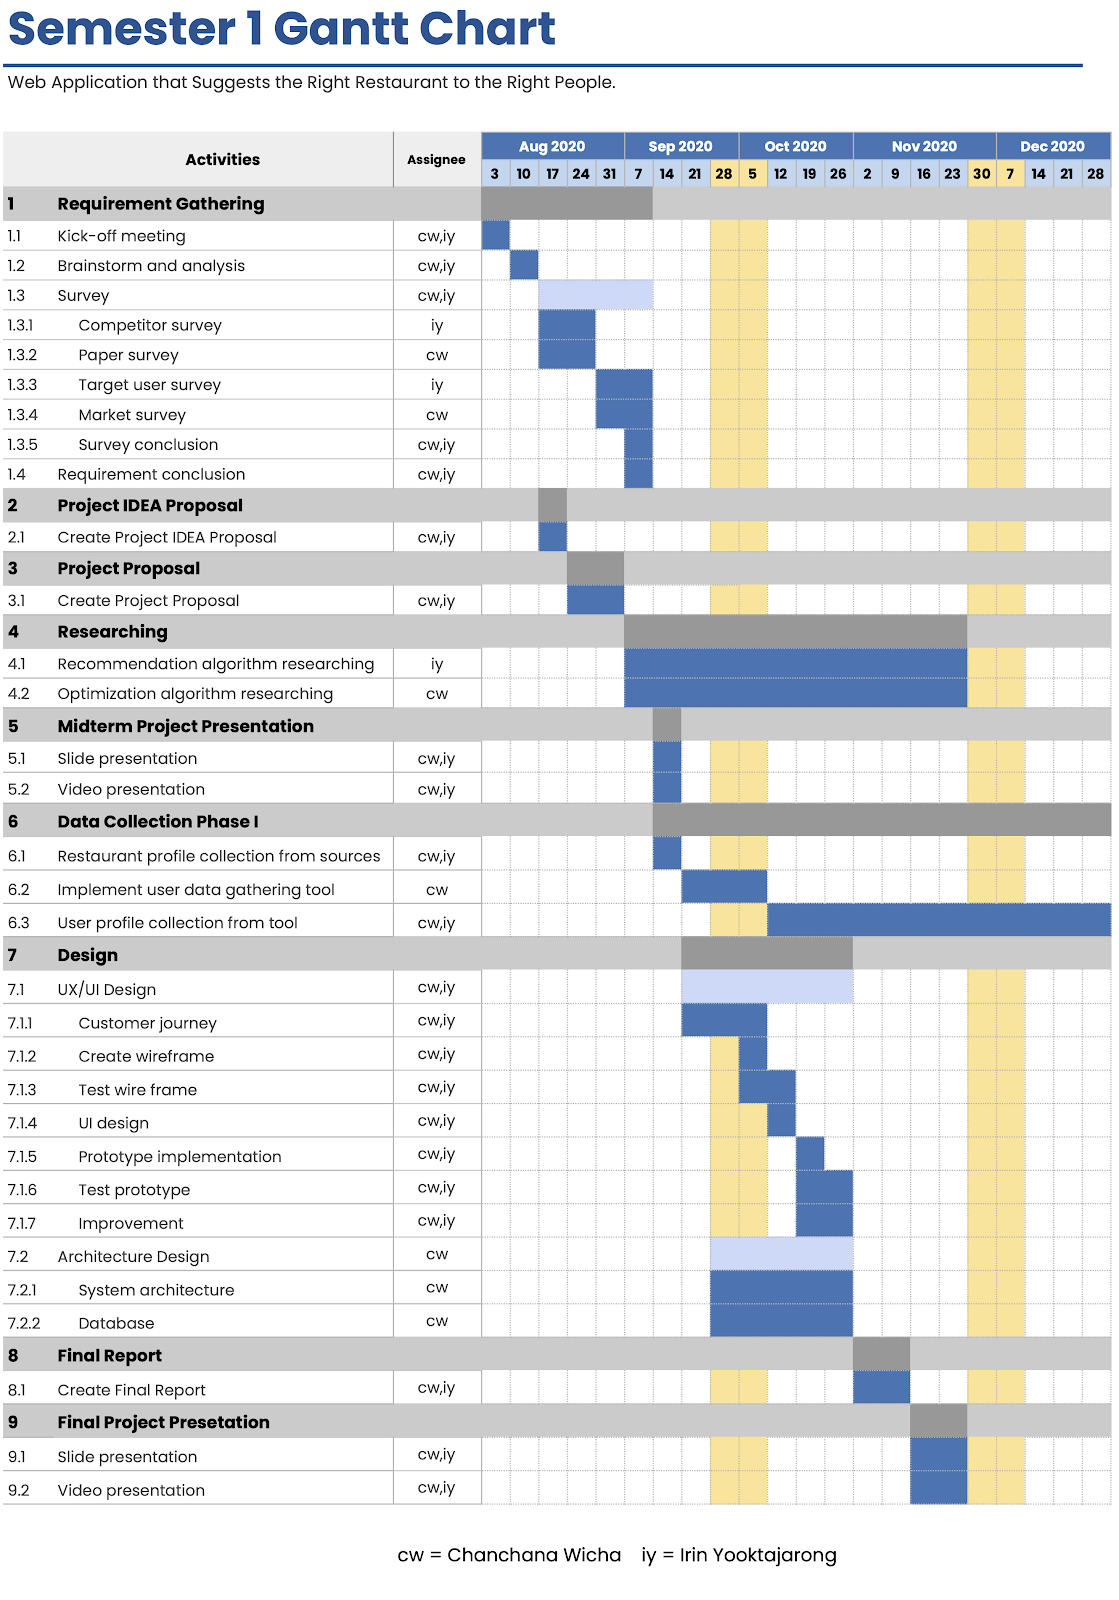
\includegraphics[width=440pt]{./images/1gantt1.png}
\caption{Gantt Chart for the First Semester}\label{fig:1_1}
\end{figure}

\begin{figure}[!h]\centering
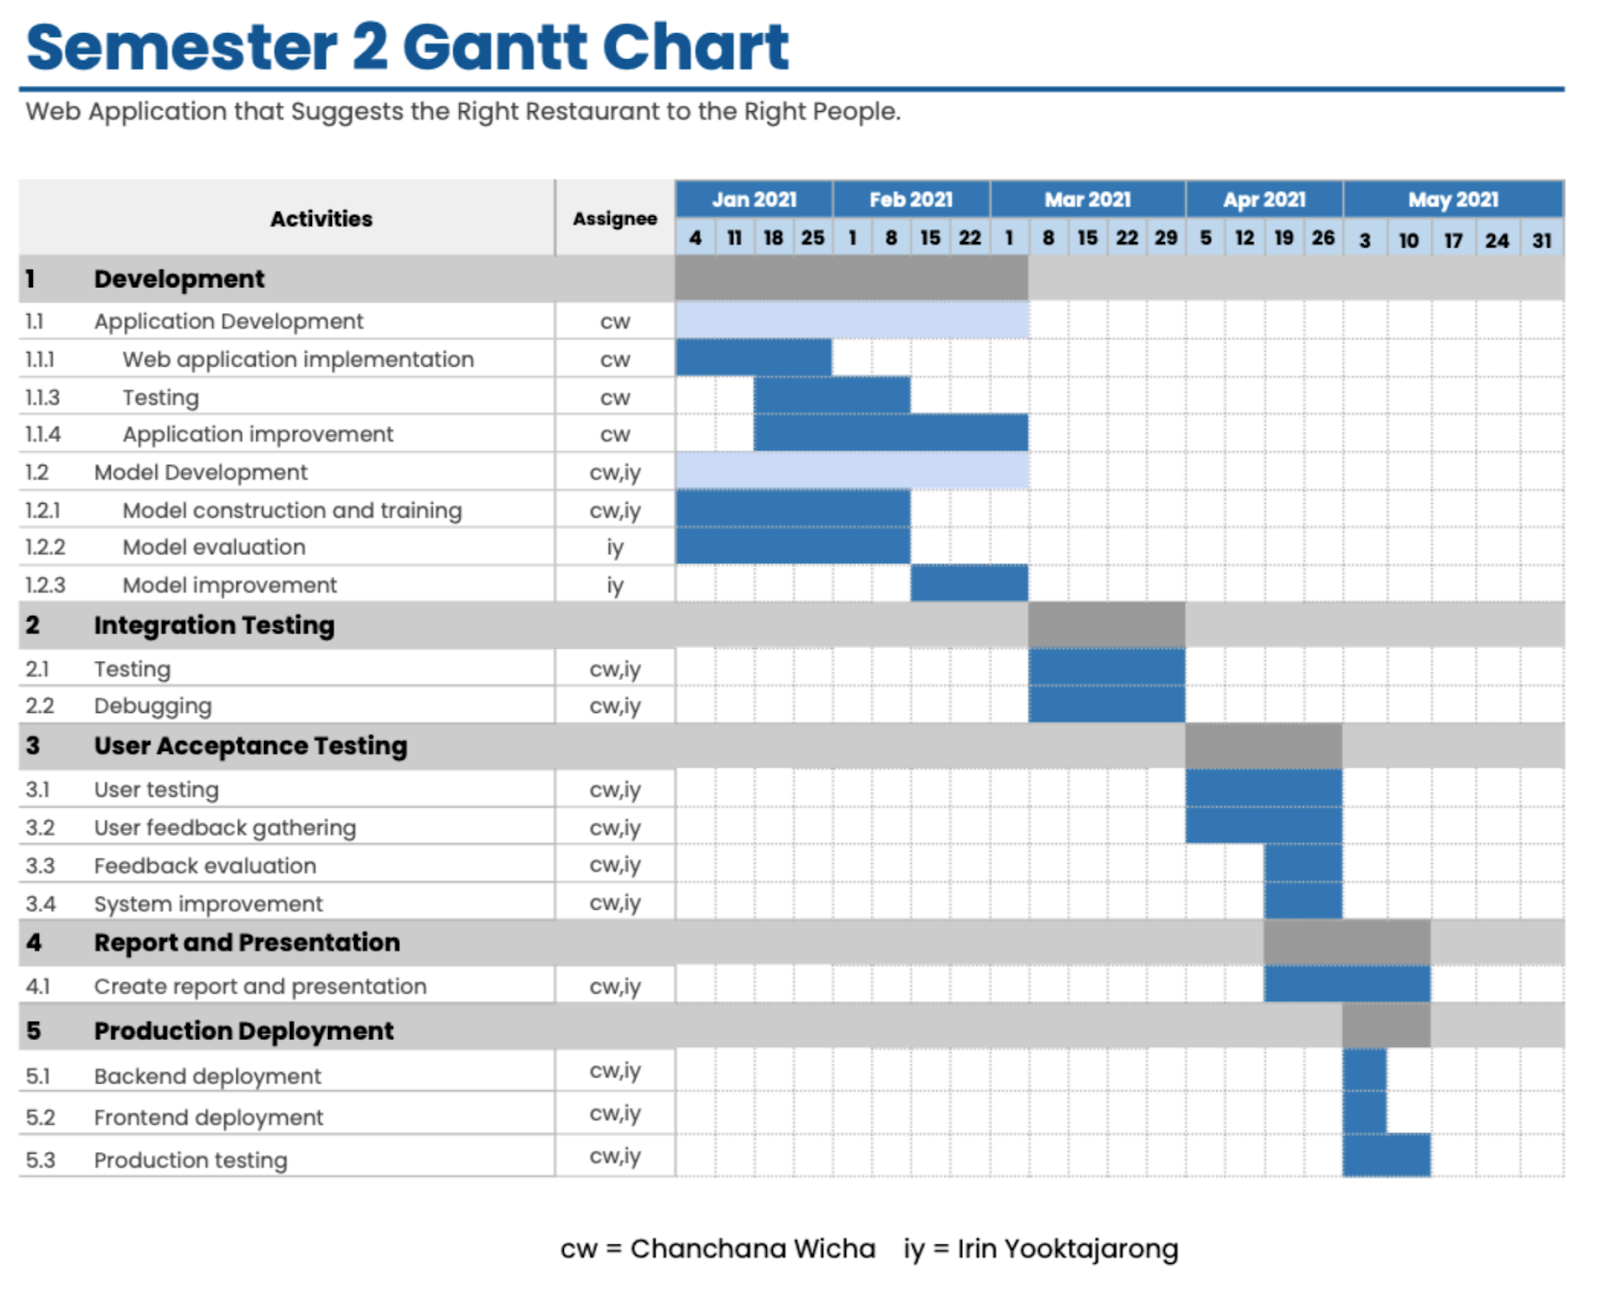
\includegraphics[width=440pt]{./images/1gantt2.png}
\caption{Gantt Chart for the Second Semester}\label{fig:1_2}
\end{figure}

\newpage

\section{Deliverables for Term 1} 
\begin{itemize}
\item Requirement Specification
\item Survey Result
\item Data Collection Tool
\item Dataset (Customer Behavior and Restaurant Information)
\item Customer Journey
\item Prototype (Web Application)
\item Database Schema
\item System Architecture and Class Diagram
\item Suggestion Algorithm and Model
\end{itemize}

\section{Deliverables for Term 2} 
\begin{itemize}
\item Web Application (Frontend and Backend)
\item Recommendation System both Individuals and Groups
\item Feedback from Users
\item Application Performance Evaluation
\item Model Performance Evaluation
\end{itemize}


%%%%%%%%%%%%%%%%%%%%%%%%%%%%%%%%%%%%%%%%%%%%%%%%%%%%%%%%%%%%
%%%%%%%%%%%%%%  Literature Review %%%%%%%%%%%%%%%%%%%%%%%%%%
%%%%%%%%%%%%%%%%%%%%%%%%%%%%%%%%%%%%%%%%%%%%%%%%%%%%%%%%%%%%
\chapter{Background Theory and Related Work}

\section{Background}

As the world becomes more digital and technology is all around us, before we realized it, we were accustomed to a personalized experience. Many online businesses are implementing personalized recommendation systems that try to identify a user’s preferences and provide them with relevant items to enhance the user's experience. However, mainstream restaurant recommendation applications in Thailand have not implemented personalized recommenders yet. This leads to the issue of finding an ideal restaurant which is always struggling for users and a person who is looking for new restaurants. Furthermore, the online problem survey revealed that many people faced a harder time to decide due to the group eating. Therefore, group decision making is very complex and time-consuming.

We brought this problem up to solve it since it is a common problem that everyone faces in daily life and no solution can be solved sustainably. Moreover, the majority of recommender systems are designed for individual users and the group recommender is challenging and new in the market. Inspired by such a challenge, we will invent a restaurant recommender system that could potentially reduce decision-making time for both individuals and groups and be an alternative way for users to opt for their ideal restaurants. Our system considers the interaction between users and restaurants and also uses side information e.g. users’ tastes and preferences, restaurant profile, etc. This approach is able to maximize users’ satisfaction and increase users’ experience.


\section{Related Theory}

\subsection{Web Application}

A web application is an application program that is stored on a remote server and delivered over the internet through a browser interface. \cite{WhatIsWebApplicationWebAppsAndItsBenefits} Because web applications are delivered through the internet, users do not need to install the application and it also allows multiple users access to the application at the same time on the same version. Moreover, running web applications require only an internet browser, so a web application is a platform and operating system independent.

Because our platform needs to be easily accessible for users not only individual users but also every member in the group of users, having a web application that does not require any installation and platform independence is a perfect solution. Users can easily access our platform via their mobile internet browser and all of them will see the same version of the application. A web application also accommodates the development process since we do not need to implement the different versions for different platforms.


\subsection{Information Collection}

This collects relevant information of users to generate a user profile or model for the prediction tasks including the user’s attributes, behaviors, or content of the resources the user accesses. \cite{WhatisMachineLearning} We need to do this process due to the recommender cannot provide results accurately until the users’ profile and preferences have been constructed. So, there are several types of information/feedback that can be captured and studied including explicit and implicit feedback.


\subsubsection{Explicit Feedback}

The accuracy of the recommendation depends on the number of ratings provided by the user. The only shortcoming of this method is, it requires effort from the users and also, users are not always ready to supply enough information. Despite the fact that explicit feedback requires more effort from the user, it is still seen as providing more reliable data, since it does not involve extracting preferences from actions, and it also provides transparency into the recommendation process that results in a slightly higher perceived recommendation quality and more confidence in the recommendations. \cite{Recommendersystem}

\subsubsection{Implicit Feedback}

The system automatically infers the user’s preferences by monitoring the different actions of users such as the history of purchases, navigation history, and time spent on some web pages, links followed by the user, content of an email, and button clicks among others. Implicit feedback reduces the burden on users by inferring their user’s preferences from their behavior with the system. The method though does not require effort from the user, but it is less accurate. Also, it has been argued that implicit preference data might in actuality be more objective, as there is no bias arising from users responding in a socially desirable way. \cite{Recommendersystem}


\begin{table}[!h]
\caption{Characteristics of Explicit and Implicit Feedback}\label{tbl:2CharacteristicsofExplicitandImplicitFeedback}
\begin{tabular}{l|l|l} \hline\hline
Implicit Feedback & Explicit Feedback & Accuracy \\ \hline\hline
Low & High & Abundance \\ \hline
High & Low & Context-sensitive \\ \hline
Yes & Yes & Expressivity of user preference \\ \hline
Positive & Positive and Negative & Measurement reference \\ \hline
Relative & Absolute \\ \hline\hline
\end{tabular}\par
\smallskip
Source: https://core.ac.uk/download/pdf/207051652.pdf
\end{table}


From Table~\ref{tbl:2CharacteristicsofExplicitandImplicitFeedback}, the accuracy of implicit feedback is lower than explicit feedback due to system monitoring only (indirect way). But with this approach, we can get abundant feedback whereas explicit feedback is scarce. Moreover, implicit feedback can capture only positive e.g. if a user never visits restaurant A that does not mean he/she does not like that restaurant. Although implicit feedback tends to be relative such as if a user visited restaurant B 10 times and restaurant C 100 times, then we can conclude that he/she has a higher preference for C than B. Lastly, as we can see from the table, one thing that is similar to each other is both are sensitive to the context


%TODO check update
In this project, the PDPA or Personal Data Protection Act is not related to us. This rule mentioned about the protection of personal information. Any app that needs access to that data needs consent from the owner by informing the purpose of what information is collected and using that information for what purpose. However, we collected user information including username, password, and user profile: food preference where all of them do not relate to personal information.

\subsection{Overview of Machine Learning}

Machine learning is an application of artificial intelligence (AI) that provides systems’ ability to automatically learn and improve from experience without being explicitly programmed. \cite{WhatisMachineLearning} Machine learning is often categorized into 3 types which are supervised learning, unsupervised learning, and reinforcement learning.

In supervised learning, it is learned from the labeled data and predicts the future events from the labeled e.g. classified cats and dogs. In contrast, unsupervised learning deals with unlabeled data which is extremely useful to discover patterns, not just predict the future from labeled data e.g. customer segmentation. Last is reinforcement learning which is the closest to human learning by learning to take corrective action with the provided environment, for example, AlphaGo which lets the machine learn how to play Go.

As our project is a recommendation system that needs to predict the next user-preferred restaurants from interactions and side information which mainly are unlabelled data. So, the model works on its own to discover patterns and information which is the restaurant for each user based on preferences. In addition, this project is an unsupervised learning problem.


\subsection{Recommendation System Techniques}

Recommender systems are usually as if a decision making strategy that helps users select the interest items based on users’ preferences or profile from overwhelmed available items or complex environments. There are 3 main types of recommendation filtering techniques which are content-based, collaborative, and hybrid. Each of these has different features and potentials.

\subsubsection{Content-based Filtering Technique}

Content-based filtering is a technique which recommends based on the similarity between the items and using users’ profile/description. Items that are mostly related to the positive user’s evaluation are recommended to the user. This approach uses a variety of models to find the similarity document to get meaningful suggestions by treating the recommendation as a user-specific classification problem by classifying for the user's likes and dislikes based on an item's features. \cite{Collaborativefiltering} Moreover, it does not require other users’ profiles as they do not affect recommendations, for example, the system wants to recommend the product which is similar to the product that user has purchased in the past, so they use content-based filtering to be the recommender by using the characteristics of the product to recommend including genre, price, style, description, picture, etc.

Therefore, this technique has the ability to recommend new items even if there is no user’s evaluation/rating. This would mean that it is able to recommend accurately without user preferences which consequence that if there is a poor description of items and an unorganized user profile, it can lead to the worst recommendation. So, the effectiveness of the content-based filtering technique depends on the richness of descriptive information, but lastly, it is unable to recommend a product that is very different from the product that the user previously purchased, resulting in the user receiving a not diverse category of product. To overcome this, it can adapt to some form of a hybrid system.

Moreover, from this approach, our project can use the algorithm to be part of our recommendation system which makes the system have an ability to recommend a restaurant even if there’s no user preference or we can say that we are able to overcome the new user problem.


\subsubsection{Collaborative Filtering Technique}

\begin{figure}[!h]\centering
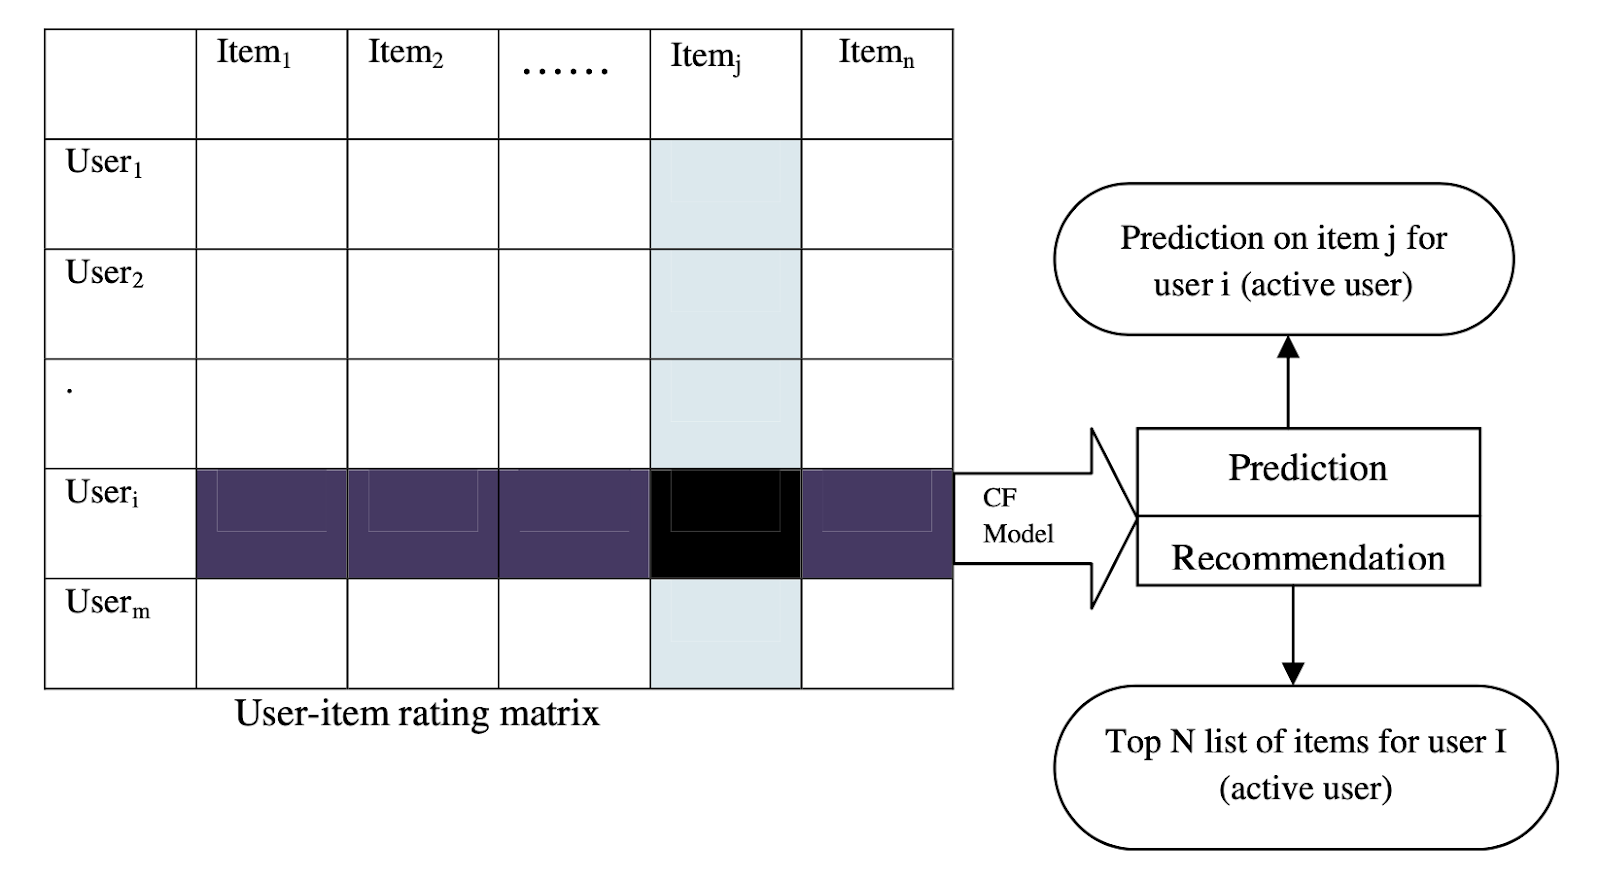
\includegraphics[width=250pt]{./images/2cfprocess.png}
\caption{Collaborative Filtering Process}\label{fig:2cfprocess}
\end{figure}

A collaborative filtering technique as opposed to the content-based filtering technique which collaborative filtering cannot recommend the item by using only the description of metadata. The key idea of this technique is a group of people with similar tastes, often tend to like similar items. So, collaborative filtering uses only data about rating profiles from different users or items in order to generate the recommendation. Here is the flow of this technique:

\begin{enumerate}
\item Gather user expression from her/his preferences by items rated.
\item Match the user’s ratings with other users’ then find the most similar tastes.
\item Recommend with the high rating of unseen items from similar users to this user.
\end{enumerate}

To recommend, it works by creating a user-item matrix of preferences for items by users, as Figure~\ref{fig:2cfprocess} above which represents the process start from the matrix to the output of this system, and then calculating the similarity between profiles to get the relevant item that matches the user. Thus, the user will be able to get the items that he/she has not rated yet but already rated from a similar user. This approach can produce the output either prediction or recommendation by prediction represented as a score of an item for the user whereas recommendation is represented as a top N list of items as mentioned in Figure~\ref{fig:2cfprocess}. Collaborative filtering techniques can separate into 2 main categories: memory-based and model-based.


\paragraph{Memory-based}\

Memory-based can approach in 2 ways which are user-based and item-based.

User-based collaborative filtering is to find the users who are similar to the target user and then recommend by calculating the weighted averages of the ratings from the group of similar users. For item-based collaborative filtering is calculating the similarity between items instead of users for determining the items which are similar to the target item then, calculating the weighted average of the ratings from a group of similar items.

To calculate the weighted average, there are several popular similarity measurements to find the similarity between user/item including Pearson correlation coefficient and Cosine similarity.

\begin{equation}\label{eq:simil}
simil(x, y) = \frac{\sum_{i\in I_xy}^{}(r_{x,i}-\bar{r}_{x})(r_{y,i}-\bar{r}_{y})}
{\sqrt{\sum_{i\in I_xy}^{}(r_{x,i}-\bar{r}_{x})^2}\sqrt{\sum_{i\in I_xy}^{}(r_{y,i}-\bar{r}_{y})^2}}
\end{equation}

From the above example equation~\ref{eq:simil}, it is a Pearson correlation coefficient, $simil(x, y)$ denotes the similarity between 2 users $x$ and $y$, mean the rating given to the item $i$ by user $x$, $\bar{r}_{x}$ means the mean rating of user $x$, $I_{xy}$ and is equal to a total number of items in the user-item.


\begin{equation}\label{eq:cos}
cos(\vec{x},\vec{y}) 
=\frac{\vec{x}\cdot \vec{y}}{\left \| \vec{x} \right \|\times \left \| \vec{y} \right \|}
=\frac{\sum_{i\in I_xy}^{}r_{x,i}r_{y,i}}
{\sqrt{\sum_{i\in I_xy}^{}r_{x,i}^2}\sqrt{\sum_{i\in I_xy}^{}r_{y,i}^2}}
\end{equation}

For cosine similarity~\ref{eq:cos}, it is different from Pearson correlation coefficient which calculates as a vector-space model by measuring the similarity between dimensional vectors based on the angle which $cos(\vec{x},\vec{y})$ denotes to the similarity between 2 users $x$ and $y$.


\paragraph{Model-based}\

This approach is able to improve the performance of collaborative filtering by constructing the model which is done by using machine learning or data mining techniques. Moreover, with this approach, dimensionality reduction methods are mostly being used as complementary techniques to improve the robustness and accuracy of the memory-based approach. \cite{Recommendersystem}

For example, this technique is matrix factorization which is able to discover hidden concepts and their relationship with users and items.

\

The advantage of the collaborative filtering technique is performed in domains where there is not much content associated with items and where content is difficult for a computer system to analyze such as opinions and ideas. \cite{Recommendersystem} But there is some disadvantage which is about the cold-start problem which refers to the new user or item that comes with the empty profile since the user has not rated any item yet. Moreover, a memory-based approach has a problem with scalability. This issue can be solved by the model-based approach.

Collaborative filtering can perform better than content-based filtering in poor content. With the advantages of this technique, we are able to reduce the user effort by performing with the implicit feedback that comes from the system monitoring and get the recommendation result more accurately.


\subsubsection{Hybrid Filtering Technique}

The hybrid filtering technique is the most recommender system used nowadays. It is a combination of content-filtering, collaborative filtering, and other approaches. There are several ways to implement e.g. doing content filtering and collaborative filtering predictions separately and then combining them later, etc. Combining different recommendation techniques can provide a better system and be able to overcome the limitations of a pure recommendation system.

Therefore, the Hybrid approach can give a better recommendation than a pure approach and can avoid the cold-start problem, sparsity, scalability, and other problems.

According to both techniques which are content-based and collaborative filtering, we found that they can reduce both of their problems whether cold-start problems that come from collaborative filtering which are content-based able to overcome, or about the diversity recommendation problem which hybrid approach can overcome. In our opinion, the hybrid filtering technique is the best choice to be done in a restaurant recommendation system.
        
        

\subsection{Aggregation Mechanism}

Since this project aims to recommend the restaurant to users both individuals and groups, we need to aggregate individual preferences into group preferences before recommending to a group of users. There are many existing strategies for aggregation but the key idea of this approach is how the individual group members’ preferences are combined into a group preference.

For the aggregating preferences strategy, the individual preferences will be aggregated into groups by combining the user’s preferences/ratings of each item and let this be the group rating. Then, group recommendations will be based on this preference and offer only the top N recommendations list to the group which N refers to the number of items that will be recommended to a group.

\subsection{Optimization Techniques}

The optimization algorithm is a procedure which is executed iteratively by comparing various solutions till an optimum or a satisfactory solution is found \cite{AlgorithmsforDiscreteOptimization} which can be either the minimum or the maximum value. The optimal value can be selected from a set of available solutions with some criterion \cite{Mathematicaloptimization}. Examples of objective functions that require maximum values ​​are: number of kilometers that a delivery vehicle can run per 1 gallon of fuel, number of customers, number of customers eating in a restaurant per hour, etc. Examples of objective functions that require minimum values ​​are: cost per unit of production, factory electricity consumption per hour, and so on.

In this project, we have adopted a method of optimization to define the objective function of our system. The objective of our system is to maximize the satisfaction of users based on the recommendations of restaurants that meet the interests and needs of that user.

\subsection{Genetic Algorithm}

The genetic algorithm (GA) is a metaheuristic method inspired by the process of natural selection that belongs to the larger class of evolutionary algorithms (EA). Genetic algorithms are commonly used to generate high-quality solutions to optimization and search problems by relying on biologically inspired operators such as mutation, crossover, and selection. \cite{Geneticalgorithm}

In the genetic algorithm, the optimal solution is found by replacing an existing set of parameters in the form of chromosomes. Each parameter in the chromosome is known as a gene which is usually replaced with binary numbers by encoding methods. Encoding of chromosomes is the first step in solving the problem and it depends on the problem. The initial population will be random values. To find the fitness solution, each generation will either mutate or switch genes between each other until a new generation of population with more fitness is obtained, this evolving process will continue until a suitable answer is found. The overall process of genetic algorithms is shown in the following pseudocode.

%TODO use algorithm package

\textbf{Pseudocode}\cite{IntroductiontoGeneticAlgorithmsIncludingExampleCode}\\
\textbf{1} START\\
\textbf{2} Generate the initial population\\
\textbf{3} Compute fitness\\
\textbf{4} REPEAT\\
\textbf{5} \quad Parent Selection\\
\textbf{6} \quad Crossover/Mutation\\
\textbf{7} \quad Compute fitness\\
\textbf{8} UNTIL population has converged\\
\textbf{9} STOP\\

The genetic algorithm consists of 4 main phases: Initial Population, Selection, Reproduction, and Termination. The details of each phase are as follows.


\paragraph*{1. Initial Population}\

%TODO check for update
Before getting the population, the problem needs to go through the encoding methods which can be binary, permutation, or value encoding. Binary encoding is the most common method that represents the solution in strings of 1s and 0s. Permutation encoding is usually used for Travelling Salesman Problem which every chromosome is a string of numbers. Value encoding is used in the problem where complicated values and binary method would not be sufficient, so that it is necessary to develop a specific crossover and mutation method.

Population comes from the set of chromosomes which each chromosome is a solution to a problem that needs to be solved. Genes can combine to be a chromosome which is known as the solution. The value of genes is randomized, with the initial number of genes dependent on the problem and sometimes can be significantly randomized to get closer to the answer.

\paragraph*{2. Selection}\

The idea of selection is to select the appropriate chromosomes or the fitter chromosomes measured by a fitness function and pass them to the next generation to be able to get a more optimal answer to the problem. Generally, chromosomes with higher fitness have more chances than lower fitness to reproduction.

\paragraph*{3. Reproduction}\

After the selection process, this process will use those chromosomes to generate the next generation by either crossover or mutation. Crossover is the most significant phase in a genetic algorithm. For each pair of parents to be mated, a crossover point is chosen at random from within the genes. \cite{IntroductiontoGeneticAlgorithmsIncludingExampleCode} After that, offspring will be created and added to the population of next generation. For mutation, it occurs when new offspring are formed by flipped some bits. This process exists to maintain the diversity of population and prevent premature convergence.

\paragraph*{4. Termination}\cite{Geneticalgorithm}

This generational process is repeated until a termination condition has been reached. Common terminating conditions are:

\begin{itemize}
\item A solution is found that satisfies minimum criteria
\item Fixed number of generations reached
\item Allocated budget (computation time/money) reached
\item The highest ranking solution's fitness is reaching or has reached a plateau such that successive iterations no longer produce better results
\item Manual inspection
\item Combinations of the above
\end{itemize}

\

In this approach, we can create a recommendation system for both individuals and groups which is based on users’ preferences along with the user's restaurant selection history. Genetic algorithms approach is the most likely to be able to serve our objective which is to maximize the satisfaction of users.




\section{Technologies}
%TODO
\section{Related Research/Competing Solutions}
%TODO




\chapter{Methodology and Design}

\section{System Functionality}
\subsection{Requirements}
\begin{itemize}
\item Users are able to register if they do not have an account.
\item Users are able to logout from our system.
\item An individual user is able to see the suggested restaurants.
\item Users are able to set restaurant preferences for each meal.
\item Users are able to see information about restaurants.
\item Users are able to select the restaurant that they want to go from the individual recommendation.
\item Users are able to rank the restaurants that they want to go by their preference from the group recommendation.
\item Users are able to join an eating group using a group pin code.
\item A group of users is able to start a group recommendation.
\item Users are able to save restaurants to their favorites and view them later.
\item Users are able to edit their food preferences.
\item The system must recommend restaurants to individuals and groups based on their preferences and behavior.
\item The system can suggest nearby restaurants based on users’ current location.
\end{itemize}


\newpage
\subsection{Use Case Diagram}

\begin{figure}[!h]\centering
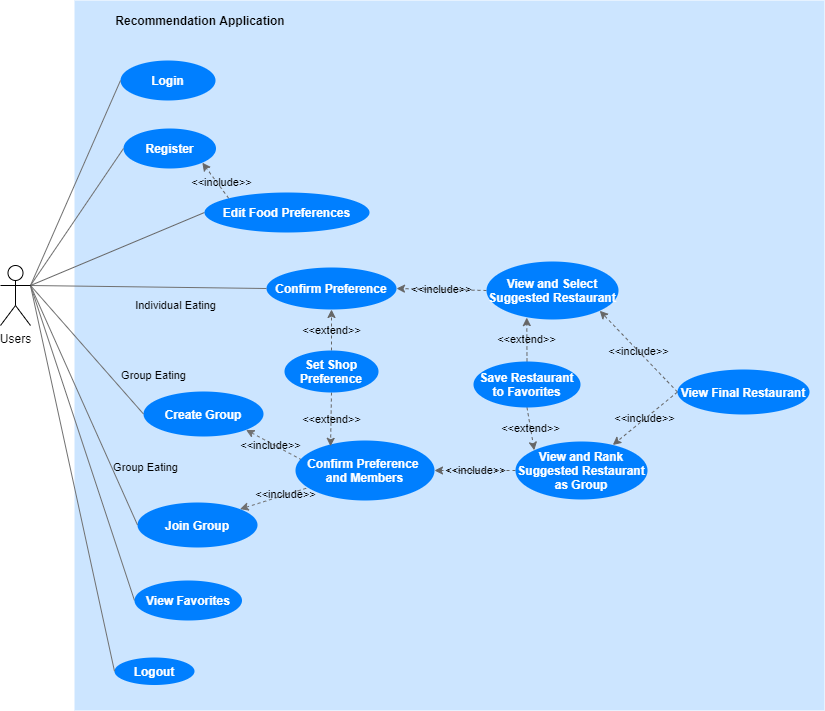
\includegraphics[width=440pt]{./images/3usecase.png}
\caption{Use Case Diagram}\label{fig:3usecase}
\end{figure}

\begin{enumerate}
\item Users can log in to the system using their username and password.
\item Users can register and users are required to set their food preference first before using the system.
\item Users can confirm the preference and see the suggested restaurants as individual eating and they can select the suggested restaurants. Moreover, users can save the restaurant into their favorite list.
\item Users can create a group or join other groups, then they can see the group confirmation page, and start the group recommendation.
\item Users can edit their food preference again.
\item Users can see their favorite list.
\item Users can log out from our system.
\end{enumerate}

\subsection{Use Case Narrative}
\subsubsection{Login}

\textbf{Name}: Users Login\\
\textbf{Actors}: Users\\
\textbf{Goal}: Users want to login into the system.\\
\textbf{Preconditions}: None\\
\textbf{Main Success Scenario}:\\
\textbf{1}. Users input their valid username and password.\\
\textbf{2}. User is logged in.\\
\textbf{Extensions (a)}\\
\textbf{1a}. Input username or password is not correct.\\
\textbf{2a}. System asks a user to input username and password again.\\
\textbf{3a}. Go back to the main scenario number 1.\\
\textbf{Extensions (b)}\\
\textbf{1b}. Input username or password is not correct.\\
\textbf{2b}. Users go to a registration page.\\
\textbf{Postconditions}: None

\subsubsection{Register}

\textbf{Name}: Users Login\\
\textbf{Actors}: Users\\
\textbf{Goal}: Users want to login into the system.\\
\textbf{Preconditions}: None\\
\textbf{Main Success Scenario}:\\
\textbf{1}. Users input their valid username and password.\\
\textbf{2}. User is logged in.\\
\textbf{Extensions (a)}\\
\textbf{1a}. Input username or password is not correct.\\
\textbf{2a}. System asks a user to input username and password again.\\
\textbf{3a}. Go back to the main scenario number 1.\\
\textbf{Extensions (b)}\\
\textbf{1b}. Input username or password is not correct.\\
\textbf{2b}. Users go to a registration page.\\
\textbf{Postconditions}: None

\subsubsection{Register}
\textbf{Name}: Users Registration\\
\textbf{Actors}: Users\\
\textbf{Goal}: Users do not have an account and want to use the system.\\
\textbf{Preconditions}: User open registration page.\\
\textbf{Main Success Scenario}: \\
\textbf{1}. System will show a general information form to the user.\\
\textbf{2}. Users fill the valid username and password in the general form.\\
\textbf{3}. Users fill all general fields in the general form.\\
\textbf{4}. Users confirm the general form.\\
\textbf{5}. System will ask the user to fill a food preference form.\\
\textbf{6}. Users fill the food preference form.\\
\textbf{7}. Users confirm the registration form.\\
\textbf{8}. User is registered and logged in.\\
\textbf{Extensions (a)} \\
\textbf{2a}. Username is invalid, already existed or password confirmation is mismatched.\\
\textbf{3a}. System asks the user to input a valid username and password again.\\
\textbf{4a}. Go back to the main scenario number 2.\\
\textbf{Extensions (b)} \\
\textbf{3b}. User didn’t fill some fields in the general form.\\
\textbf{4b}. Users confirm the general form.\\
\textbf{5b}. System asks the user to fill all the fields in the general form.\\
\textbf{6b}. Go back to the main scenario number 3.\\
\textbf{Postconditions}: None

\subsubsection{Individual Recommendation}
\textbf{Name}: Individual Recommendation\\
\textbf{Actors}: Users\\
\textbf{Goal}: Users want the system to suggest restaurants for them.\\
\textbf{Preconditions}: User is logged in and opens an individual recommendation page.\\
\textbf{Main Success Scenario}: \\
\textbf{1}. User allows the system to access their current location\\
\textbf{2}. The system shows a confirmation page to the user.\\
\textbf{3}. Users confirm the setting.\\
\textbf{4}. The system will show the suggested restaurant to the user\\
\textbf{5}. Users select the restaurant that they want to go to.\\
\textbf{6}. Users see their selected restaurant as a final restaurant.\\
\textbf{7}. Recommendation completed\\
\textbf{Extensions (a)} \\
\textbf{1a}. Users do not allow the system to access their current location.\\
\textbf{2a}. The nearby restaurant suggestion will be disabled.\\
\textbf{3a}. Continue to the main scenario number 2.\\
\textbf{Extensions (b)} \\
\textbf{2b}. Users change the setting for that meal.\\
\textbf{3b}. Go back to the main scenario number 3.\\
\textbf{Extensions (c)} \\
\textbf{4c}. Users save the restaurant to their favorite list.\\
\textbf{5c}. Go back to the main scenario number 5.\\
\textbf{Postconditions}: None

\subsubsection{Group Recommendation}
\textbf{Name}: Group Recommendation\\
\textbf{Actors}: Users\\
\textbf{Goal}: Users want the system to suggest restaurants for their group.\\
\textbf{Preconditions}: Users are logged in and open a group recommendation page.\\
\textbf{Main Success Scenario}: \\
\textbf{1}. Users allow the system to access their current location.\\
\textbf{2}. Users see the confirmation page and group pin code.\\
\textbf{3}. Users share pin code or QR code to others members.\\
\textbf{4}. Every member joined.\\
\textbf{5}. Head of the party selects to start the recommendation.\\
\textbf{6}. Everybody in the group sees the same set of the restaurants.\\
\textbf{7}. Everybody selects their restaurant they want to go to by their preference.\\
\textbf{8}. Everybody finished selecting the restaurants.\\
\textbf{9}. The system shows the final restaurant to the group.\\
\textbf{9}. Recommendation completed\\
\textbf{Extensions (a)} \\
\textbf{3a}. Users choose to join the group by inputting the group pin.\\
\textbf{4a}. Group pin is invalid.\\
\textbf{5a}. Users cannot join the invalid pin group.\\
\textbf{Extension (b)} \\
\textbf{6b}. Users save the restaurant to their favorite list.\\
\textbf{7b}. Continue to the main scenario number 7\\
\textbf{Postconditions}: None

\subsubsection{Edit the Food Preference}
\textbf{Actors}: Users\\
\textbf{Goal}: Users want to edit their food preference.\\
\textbf{Preconditions}: Users are logged in.\\
\textbf{Main Success Scenario}: \\
\textbf{1}. Users choose to edit their food preference.\\
\textbf{2}. The old food preference will be shown and let users edit them.\\
\textbf{5}. User confirm the modification\\
\textbf{Postconditions}: None

\subsubsection{See the Favorite List}
\textbf{Actors}: Users\\
\textbf{Goal}: Users want to see their restaurant favorite list.\\
\textbf{Preconditions}: Users are logged in\\
\textbf{Main Success Scenario}: \\
\textbf{1}. Users choose to see their favorite list.\\
\textbf{2}. The system shows a list of their favorite restaurants to the users.\\
\textbf{3}. Users see their favorite list.\\
\textbf{Extensions (a)} \\
\textbf{3a}. Users choose to remove the restaurant from their favorite list.\\
\textbf{4a}. The restaurant is removed from their favorites list.\\
\textbf{Postconditions}: None

\subsubsection{Logout}
\textbf{Name}: Users Logout\\
\textbf{Actors}: Users\\
\textbf{Goal}: Users want to logout from the system.\\
\textbf{Preconditions}: Users are logged in.\\
\textbf{Main Success Scenario}: \\
\textbf{1}. User choose to logout\\
\textbf{2}. User is logged out\\
\textbf{Postconditions}: None


\newpage
\subsection{Functional Breakdown Structure}
\begin{figure}[!h]\centering
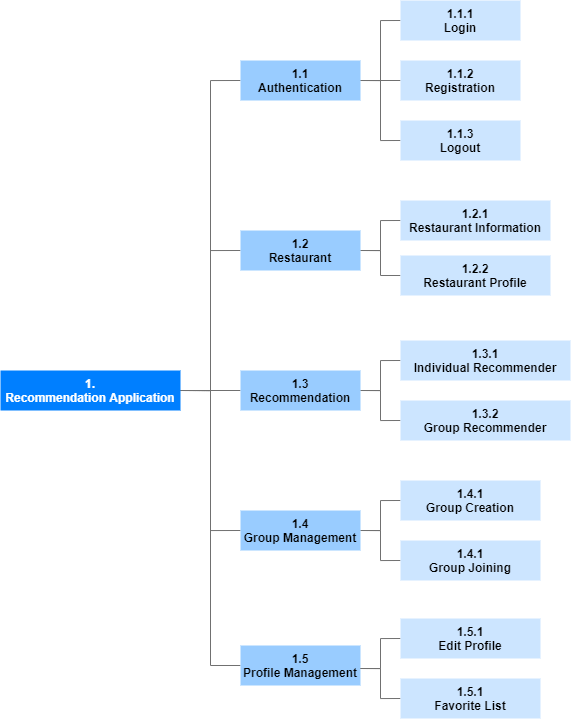
\includegraphics[width=360pt]{./images/3functional_breakdown.png}
\caption{Functional Breakdown Structure of the System}\label{fig:3functional_breakdown}
\end{figure}

Our system consists of 5 functional components which are:

\begin{enumerate}
\item Authentication, it handles user registration, login, and logout.
\item Restaurant, it serves the restaurant information and their profile which include restaurant categories, price and distance.
\item Recommendation, it generates the restaurant recommendation which is separated into individual and group recommendation.
\item Group Management, manages the group used in group recommendation.
\item Profile Management, manages the user profile and their favorite list.
\end{enumerate}


\section{System Architecture}
\subsection{System Overview}
\begin{figure}[!h]\centering
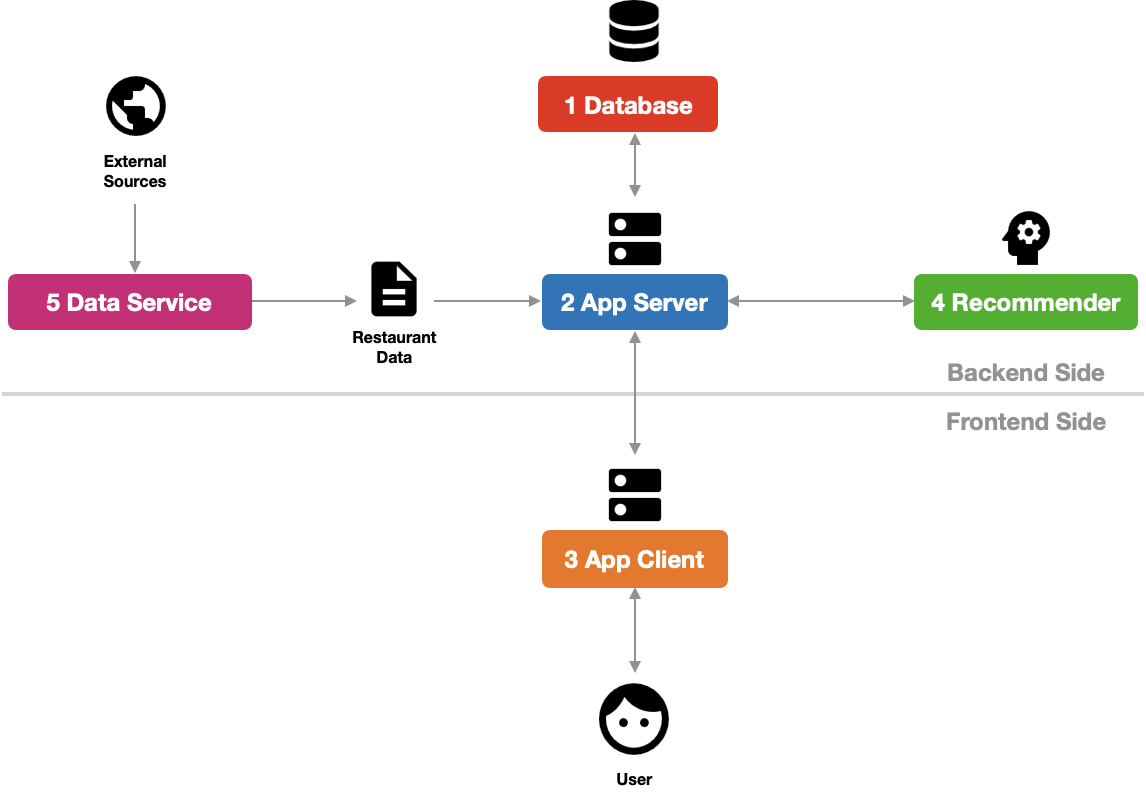
\includegraphics[width=360pt]{./images/3system_overview.png}
\caption{System Overview}\label{fig:3system_overview}
\end{figure}

In this section, we will give an overview of our system about their responsibility and we will discuss each component in detail in the next section.

From Figure~\ref{fig:3system_overview}, we can see the relationship between each component. Our system consists of mainly 5 components which are Database, App Server, App Client, Recommender, and Data Service.

%TODO Italic specific name
\begin{itemize}
\item Database: store all of the data of our system.
\item App Server: handle all server-side processes including restaurant data management, group management, recommendation request handling, and authentication system. This component acts as a center of the system.
\item App Client: serve the user interface to users via a web application.
\item Recommender: handle the restaurant's suggestion. This component will receive the recommendation request from App Server and return the suggestion result back to App Server.
\item Data Service: collect restaurant data from external sources, preprocess the data, and feed the data into App Server.
\end{itemize}

We separate these components into 2 sides which are the backend side and the frontend side. The backend side includes Database, App Server, Recommender, and Data Service. The frontend side is only App Client.


\newpage
\subsection{Restaurant Recommender System Architect}

\begin{figure}[!h]\centering
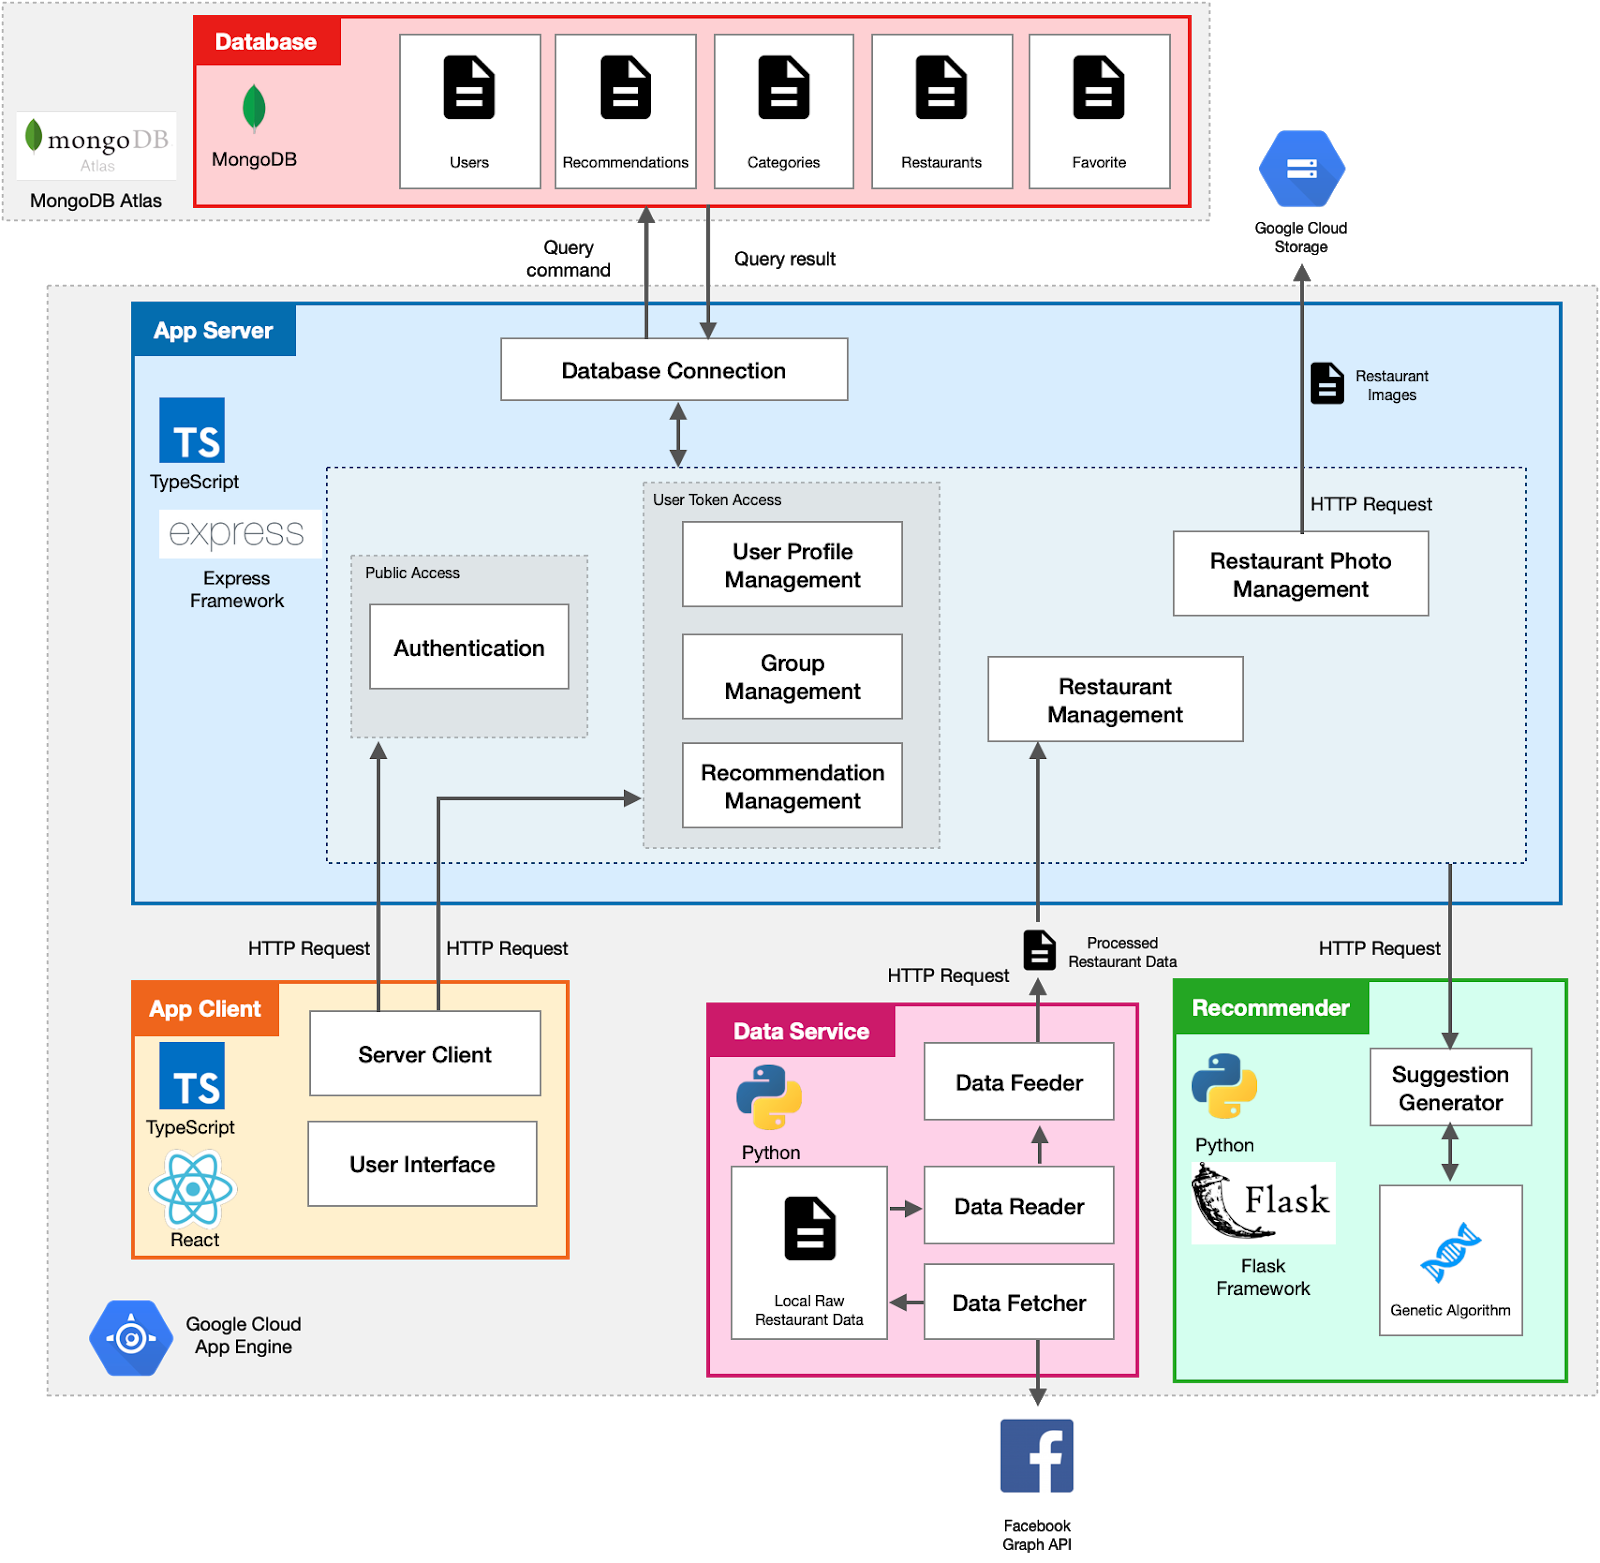
\includegraphics[width=400pt]{./images/3architect.png}
\caption{System Architecture}\label{fig:3architect}
\end{figure}

Figure~\ref{fig:3architect} shows the detailed architecture of our system. As we mentioned before, our system consists of 5 components. Each of these components communicates via HTTP request and response. All of the components except Database are deployed using Google Cloud App Engine and Database is deployed via MongoDB Atlas. There are 2 external services that our system needs to be interacted with which are Google Cloud Storage for storing restaurant’s images and Facebook Graph API for querying primary restaurant information. We will walk through each component in detail in the following section.


\newpage
\subsubsection{App Server Architecture}

\begin{figure}[!h]\centering
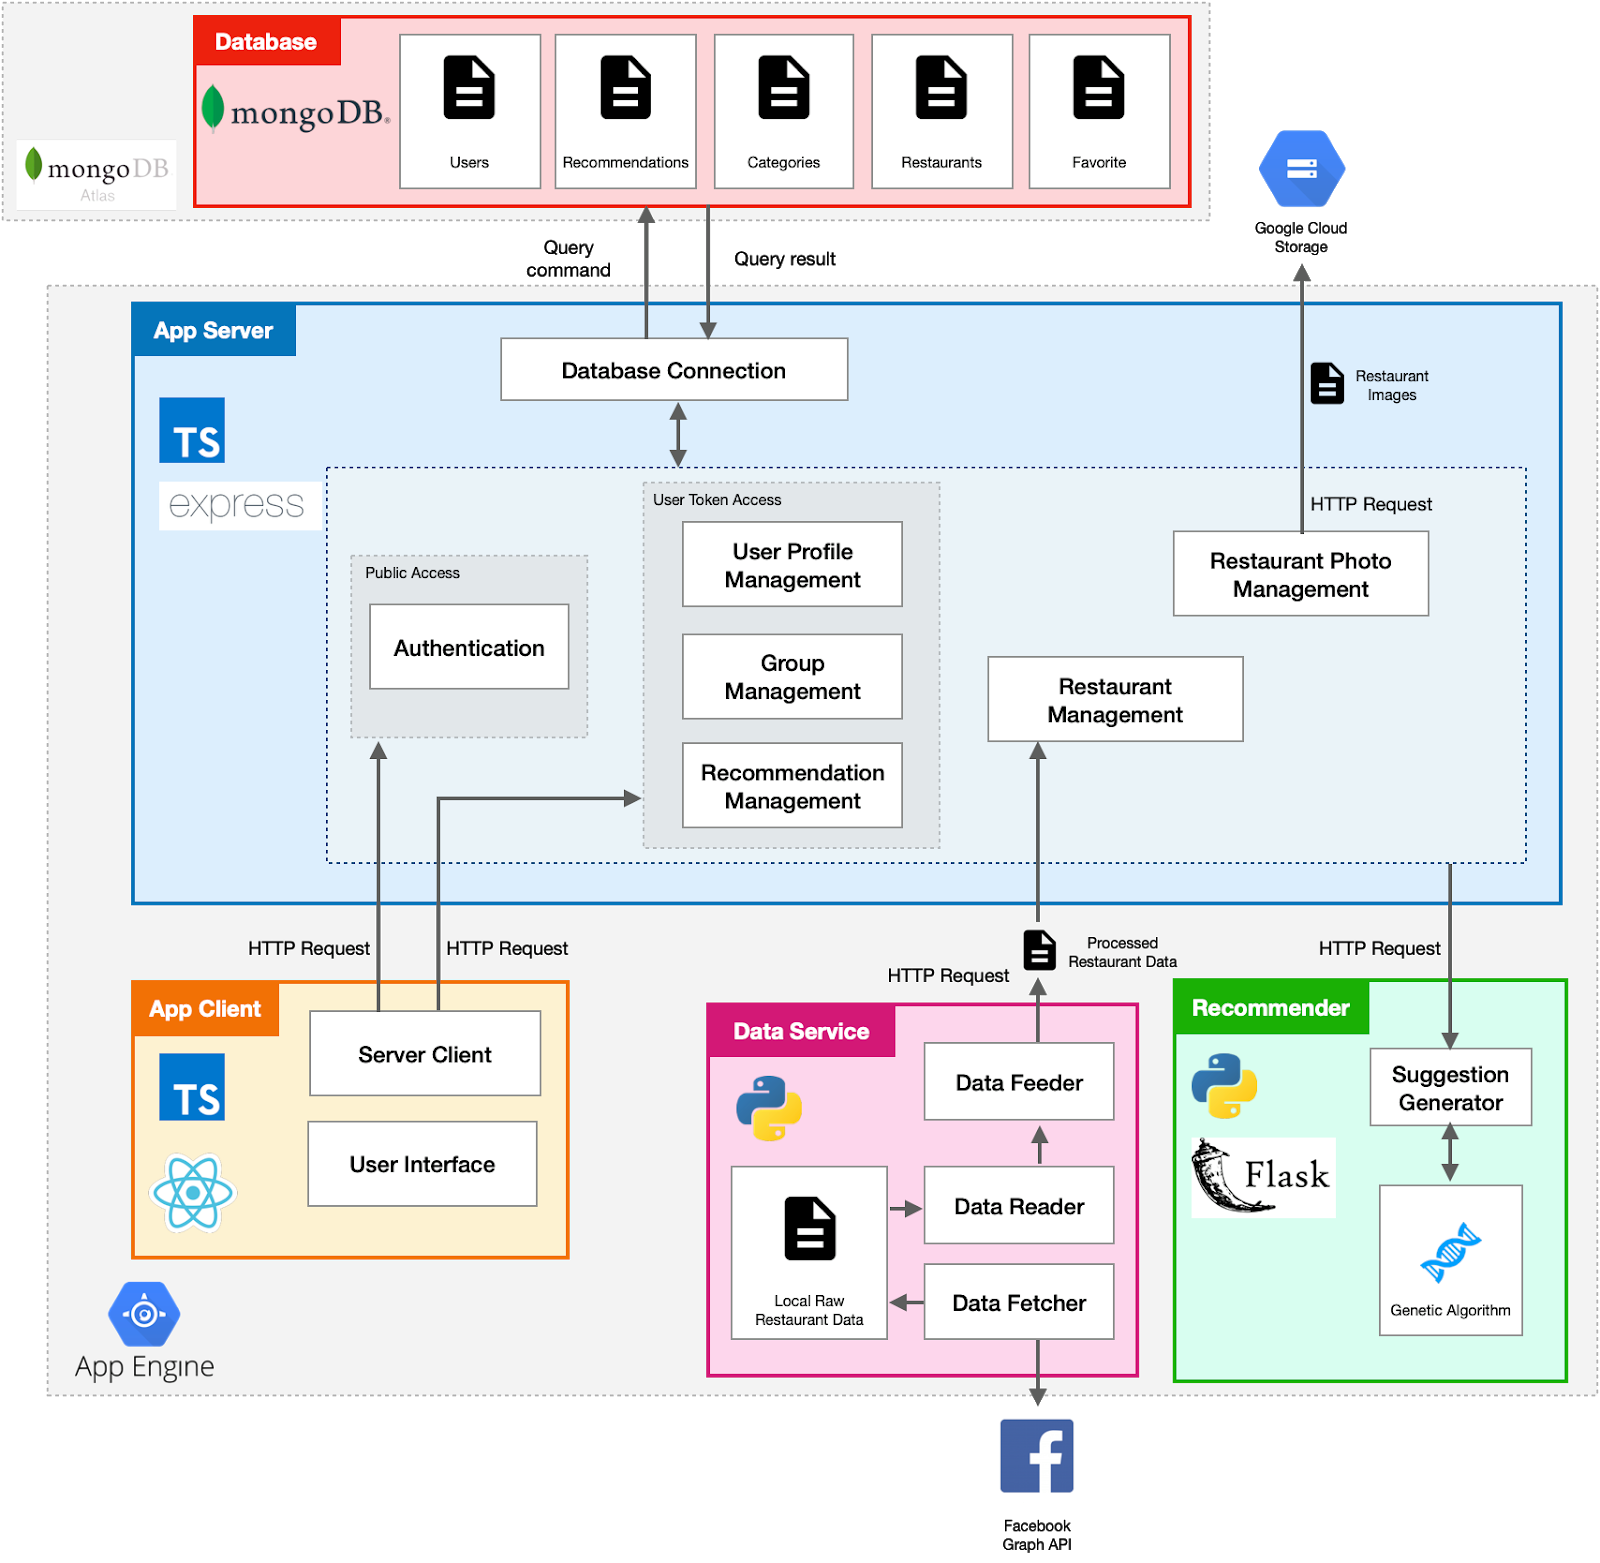
\includegraphics[width=360pt]{./images/3arch_appserver.png}
\caption{App Server Architecture}\label{fig:3arch_appserver}
\end{figure}

App Server is responsible for handling all server-side processes. The processes include authentication, user management, group management, recommendation management, restaurant management, and model management. This component acts as a center of our system that lets all other components communicate with them.

For database communication, this is the only component that allows access to the database, so any components needed to access any data must communicate through App Server. The database connection module acts as an interface to the database for App Server.

For an App Client communication, App Client needs to send a request to App Server in order to complete a task. The requests include authentication requests, create and update a recommendation request, get, create, and update group requests and get, create, and update user information requests.

For a Data Service communication, Data Service generates processed restaurant data and it sends those data to App Server to create a restaurant and store them in the database.

For a Recommender communication, App Server needs to send requests to Recommender for restaurant suggestion generation and model training. Recommender also needs to send a request to App Server to get restaurant information and user information.

There is also one external system that App Server needs to communicate with which is Google Cloud Storage. App Server will send a request to store the restaurant’s images and get the existing image from that service.

App Server is implemented using TypeScript and Express framework which is a web application framework and deployed on Google Cloud App Engine service.


\subsubsection{App Client Architecture}

\begin{figure}[!h]\centering
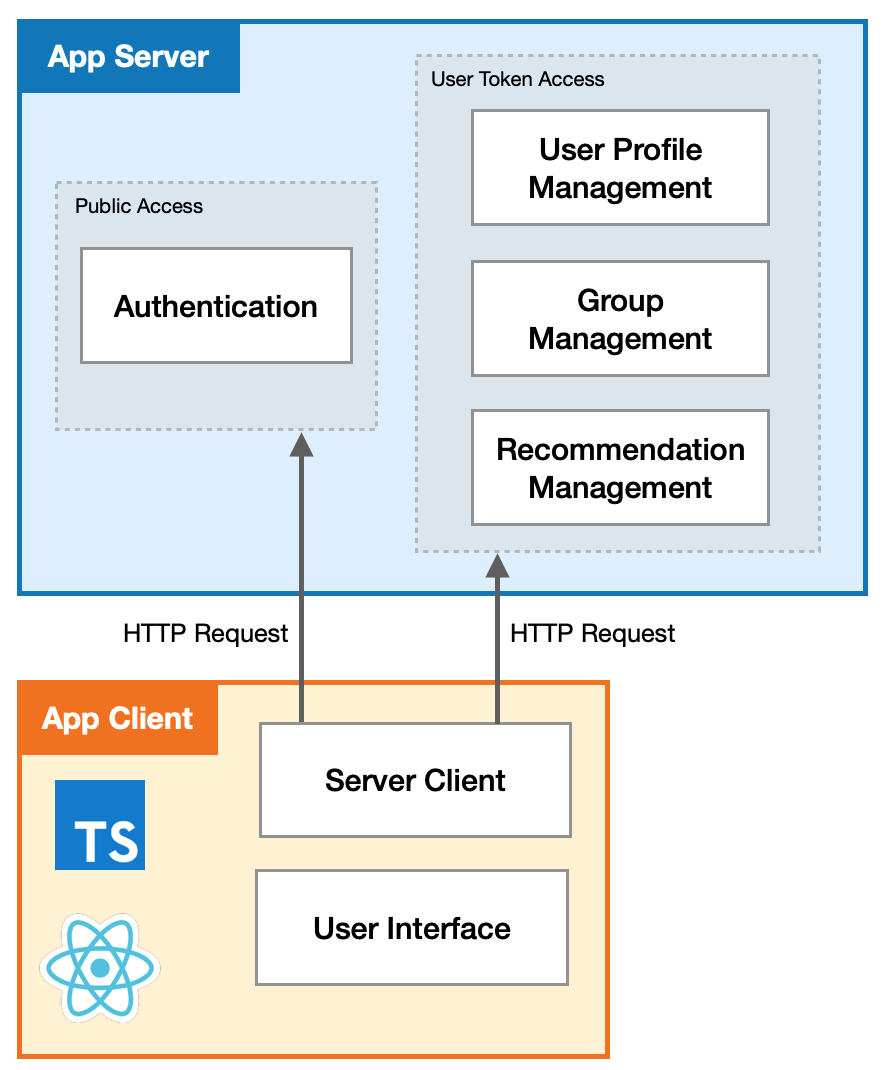
\includegraphics[width=200pt]{./images/3arch_appclient.png}
\caption{App Client Architecture}\label{fig:3arch_appclient}
\end{figure}

App Client is responsible for serving the user interface to users and handling user interactions. There are 2 modules in this component which are User Interface that serves as an interface to users and Server Client that handles user’s tasks and communicates with App Server. App Client is implemented using TypeScript and React framework and deployed on Google Cloud App Engine service.


\subsubsection{Recommender Architecture}

\begin{figure}[!h]\centering
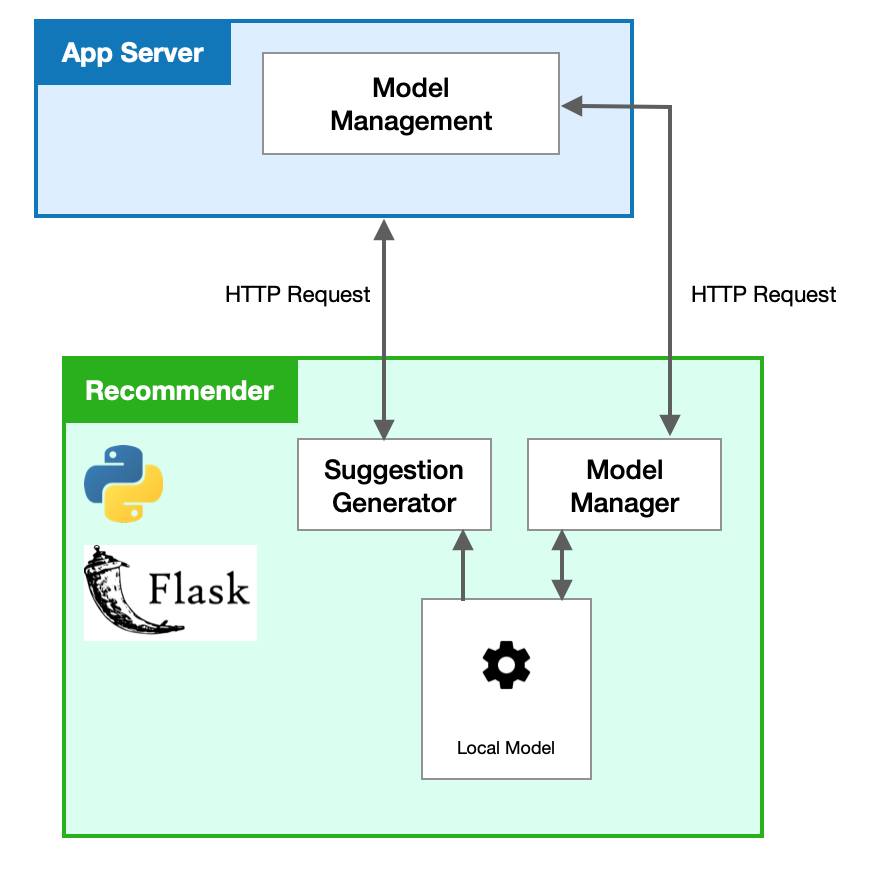
\includegraphics[width=200pt]{./images/3arch_recommender.png}
\caption{Recommender Architecture}\label{fig:3arch_recommender}
\end{figure}

Recommender is responsible for restaurant suggestion generation. There are 2 modules in this component which are Suggestion Generator and Model Manger.

Suggestion Generator will receive a recommendation request from App Server, generate one set of restaurants using a local model, and send that response back to App Server. In this process, Recommender also needs to get some information about restaurants and users from App Server for the generation.

Model Manager will manage the local model. It is waiting for a training request from App Server to train a new local model. It also sends the training information request back to App Server after the training process is finished.

Recommender implemented using Python which can easily communicate with the model because many libraries are supporting the machine learning process. It also uses the Flask framework to make them listen for requests from App Server. It is deployed on the Google Cloud App Engine service.


\subsubsection{Data Service Architecture}

\begin{figure}[!h]\centering
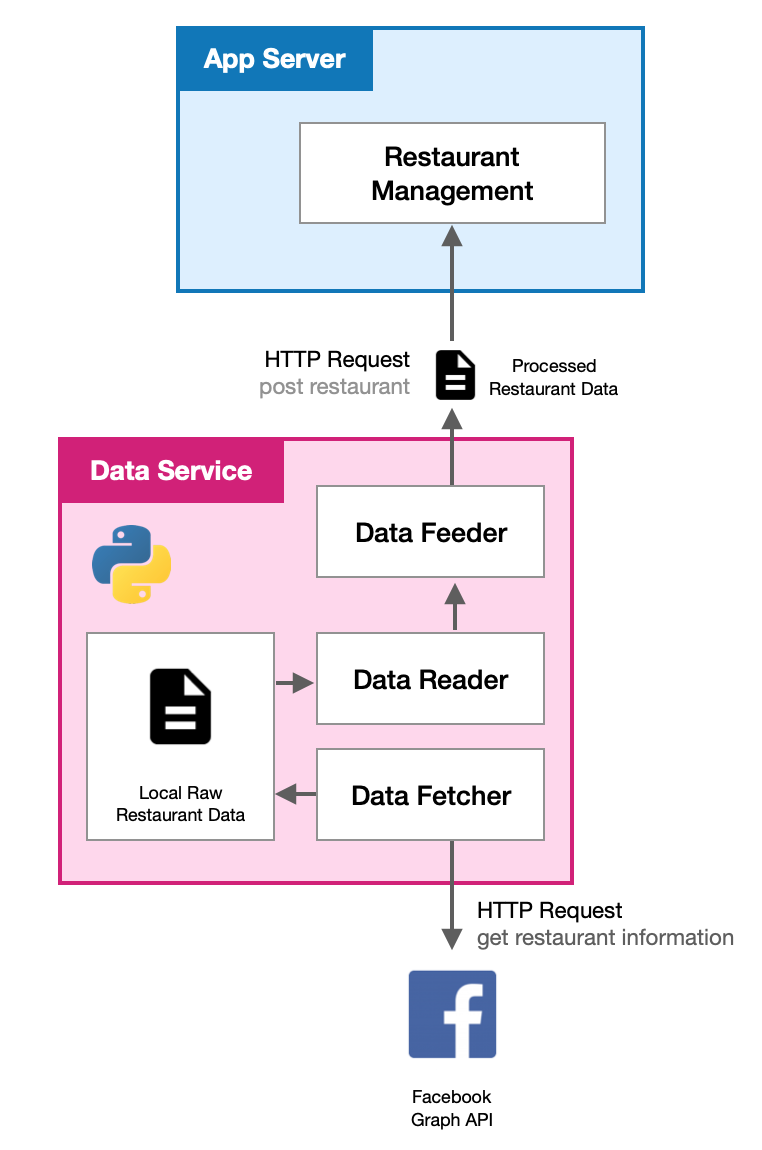
\includegraphics[width=200pt]{./images/3arch_dataservice.png}
\caption{Data Service Architecture}\label{fig:3arch_dataservice}
\end{figure}
%TODO Check for update
Data Service is responsible for collecting restaurant information from an external source. This component has 3 modules which are Data Fetcher which collect the restaurant information from Facebook Graph API and save it to the local raw files, Data Reader which will read the files and process that data into the correct format and Data Feeder will send the processed data to App Server to create restaurants in the system. Currently, it is designed to collect the restaurant data manually, so if we want to update or collect more restaurants, we need to trigger the task in this service again. Data Service is implemented as a simple Python script without any web framework because no components need to send a request to Data Service.


\subsubsection{Database Architecture}

\begin{figure}[!h]\centering
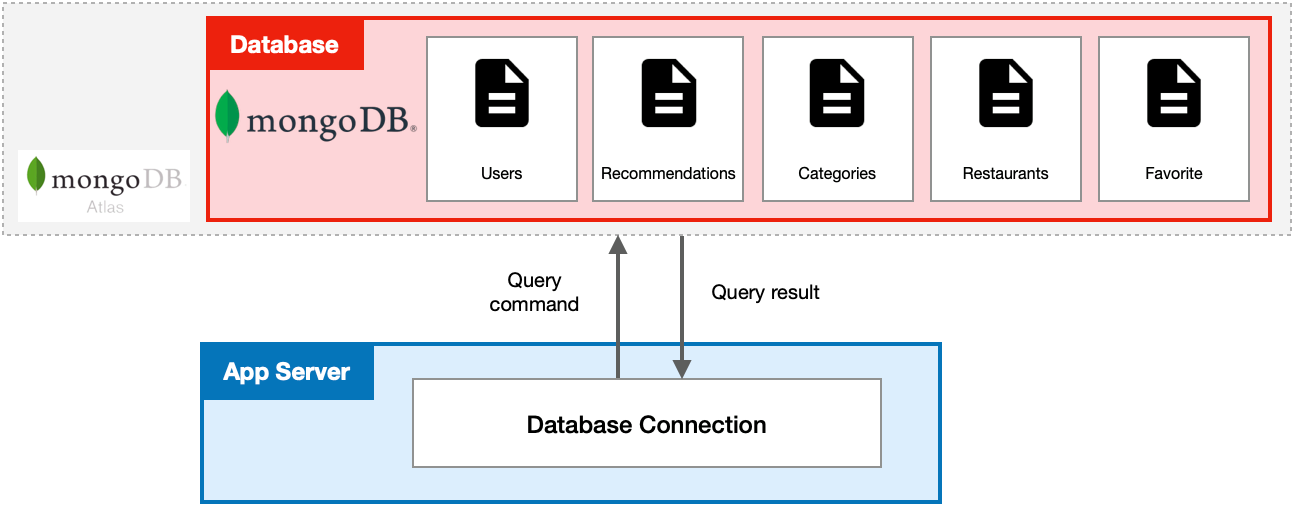
\includegraphics[width=400pt]{./images/3arch_database.png}
\caption{App Server Architecture}\label{fig:3arch_database}
\end{figure}

Database is responsible for storing all data in our system. We choose to have NoSQL for our database because the schema of the data can change quickly, having a flexible schema can make our system adapt to the change in data format more easily. We will discuss the database structure in section 3.5 Database Structure. To access the data in the database, App Server will send a query command via the database connection module in App Server. The database is implemented using MongoDB and deployed using their official cloud service, MongoDB Atlas.


\newpage
\section{User Journey}

\subsection{Activity Diagrams}

\subsubsection{Registration}

\begin{figure}[!h]\centering
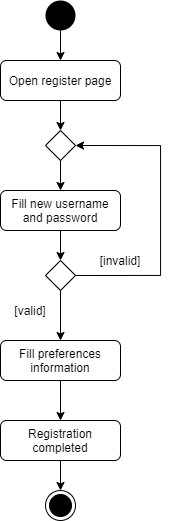
\includegraphics[height=400pt]{./images/3actdiagram_register.png}
\caption{Registration Activity Diagram}\label{fig:3actdiagram_register}
\end{figure}

When users open a registration page, they will be asked to input their new username and password. If their new username and password are valid they need to fill in the food preferences information. Then the registration will be completed.

\newpage
\subsubsection{Individual Restaurant Recommendation}

\begin{figure}[!h]\centering
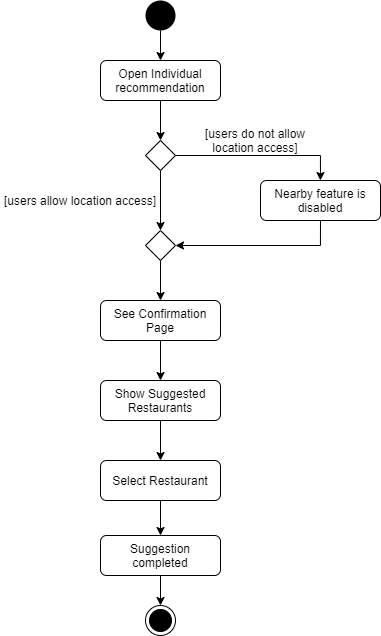
\includegraphics[height=400pt]{./images/3actdiagram_indirec.png}
\caption{Individual Restaurant Recommendation Activity Diagram}\label{fig:3actdiagram_indirec}
\end{figure}

When users choose to start the individual recommendation, users need to allow their current location access in order to use nearby suggestion features. And before entering the recommendation, they will see the confirmation page which they can configure the setting and location. After that, they will see the suggested restaurant and can optionally save any restaurant into their favorite list. If they are satisfied with the suggestion and select the final restaurant, the recommendation will be completed. Otherwise, users can choose to see more suggestions.

\newpage
\subsubsection{Registration}

\begin{figure}[!h]\centering
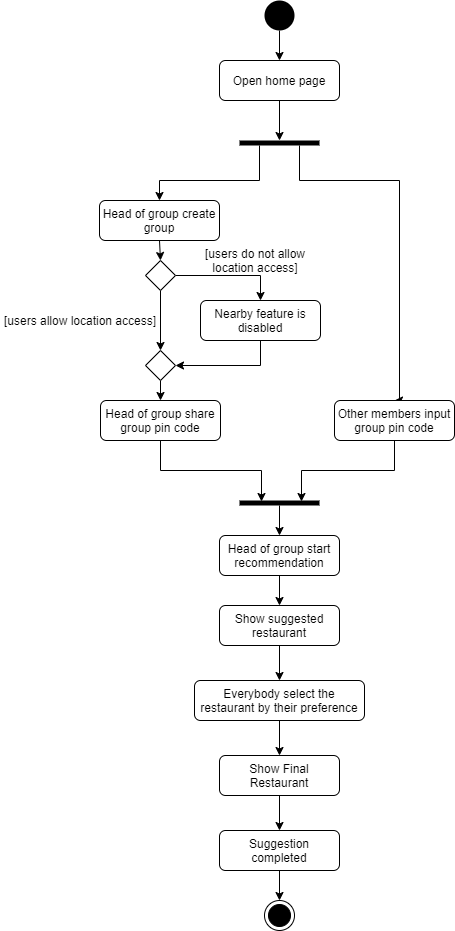
\includegraphics[height=400pt]{./images/3actdiagram_grouprec.png}
\caption{Group Restaurant Recommendation Activity Diagram}\label{fig:3actdiagram_grouprec}
\end{figure}

When a group of users wants to start a group recommendation, they firstly need to create a group and let other members join the group. This requires only one member to create a group and that person will be a head of the party which they can change the location and main configuration. Other members can use the group pin code shared by the head or other members that are already in the group. After the head chooses to start the recommendation, the same set of restaurants will be shown to all members. Everybody then needs to rank the restaurants that they want to go to by their preference. After everybody is done selecting their restaurants, the final suggested restaurant will be shown to the group and the recommendation is completed.


\newpage
\subsection{Sequence Diagrams}

\subsubsection{Registration}

\begin{figure}[!h]\centering
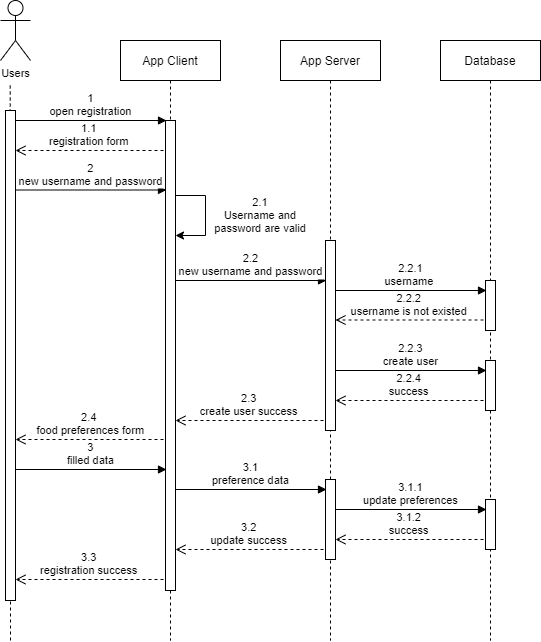
\includegraphics[height=400pt]{./images/3seqdiagram_register.png}
\caption{Registration Sequence Diagram}\label{fig:3seqdiagram_register}
\end{figure}

\textbf{Scenario}: Users register for a new account.
\begin{enumerate}
\item Users open the registration page and App Client shows the registration form to users.
\item Once users fill in their new username and password, App Client will validate the username format (2.1). If they are valid, App Client will send those fields to the app server (2.2). Next, App Server will query the username from the database (2.2.1). If the username does not exist in the database, the new user will be created (2.2.4) and sent back to App Client (2.3). The App Client will send a food preference setting form to the users (2.4).
\item Once users fill the food preferences setting form, the user profile in the database will be updated (3.1.2) and the registration will be completed (3.3)
\end{enumerate}


\newpage
\subsubsection{Individual Restaurant Recommendation}

\begin{figure}[!h]\centering
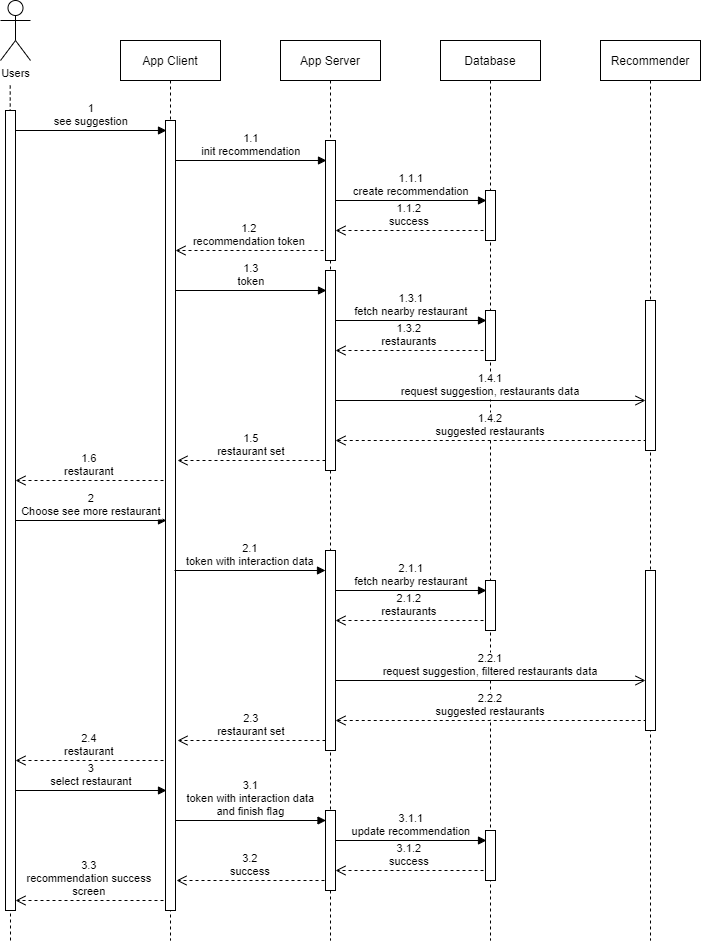
\includegraphics[height=600pt]{./images/3seqdiagram_indirec.png}
\caption{Individual Restaurant Recommendation Sequence Diagram}\label{fig:3seqdiagram_register}
\end{figure}

\newpage
\textbf{Scenario}: Users want to see the restaurant recommendation for individuals and they want to see more suggestions than the first set of the suggested restaurants.
\begin{enumerate}
\item When users want to see a recommendation, App Client will send an initial recommendation request to the App Server (1.1), App Server will create a new recommendation data (1.1.1 and 1.1.2) and send the recommendation back to App Client (1.2). Next, App Client will send the token to App Server again (1.3). Once App Server receives the token, it will fetch nearby restaurants (1.3.1 and 1.3.2) and send a recommendation request with the restaurants to Recommender (1.4.1). Recommender will generate a set of suggested restaurants and send them back to App Server and App Client (1.4.2 and 1.5). Lastly, App Client will show a restaurant in the restaurant set to users  (1.6).
\item Users will see the suggested restaurants. In this scenario, users choose to see more suggested restaurants (2). After that App Client will send a recommendation token with current restaurants interaction data to filter out the suggested restaurants in the first set (2.1). The next process is generating a restaurant suggestion which is the same process as before, but this time, App Server will send only the filtered restaurants to Recommender (2.2.1). After the suggestion is generated, it will be sent back to App Server, App Client and users (2.2.2, 2.3, and 2.4).
\item When users select the restaurant from the set (3) which means the recommendation is finished, App Client will send the recommendation token with a finish flag to App Server (3.1). App Server will send an update request to Database (3.1.1) and after its success, the recommendation success screen will be shown to users (3.3).
\end{enumerate}



\newpage

\subsubsection{Create Group}

\begin{figure}[!h]\centering
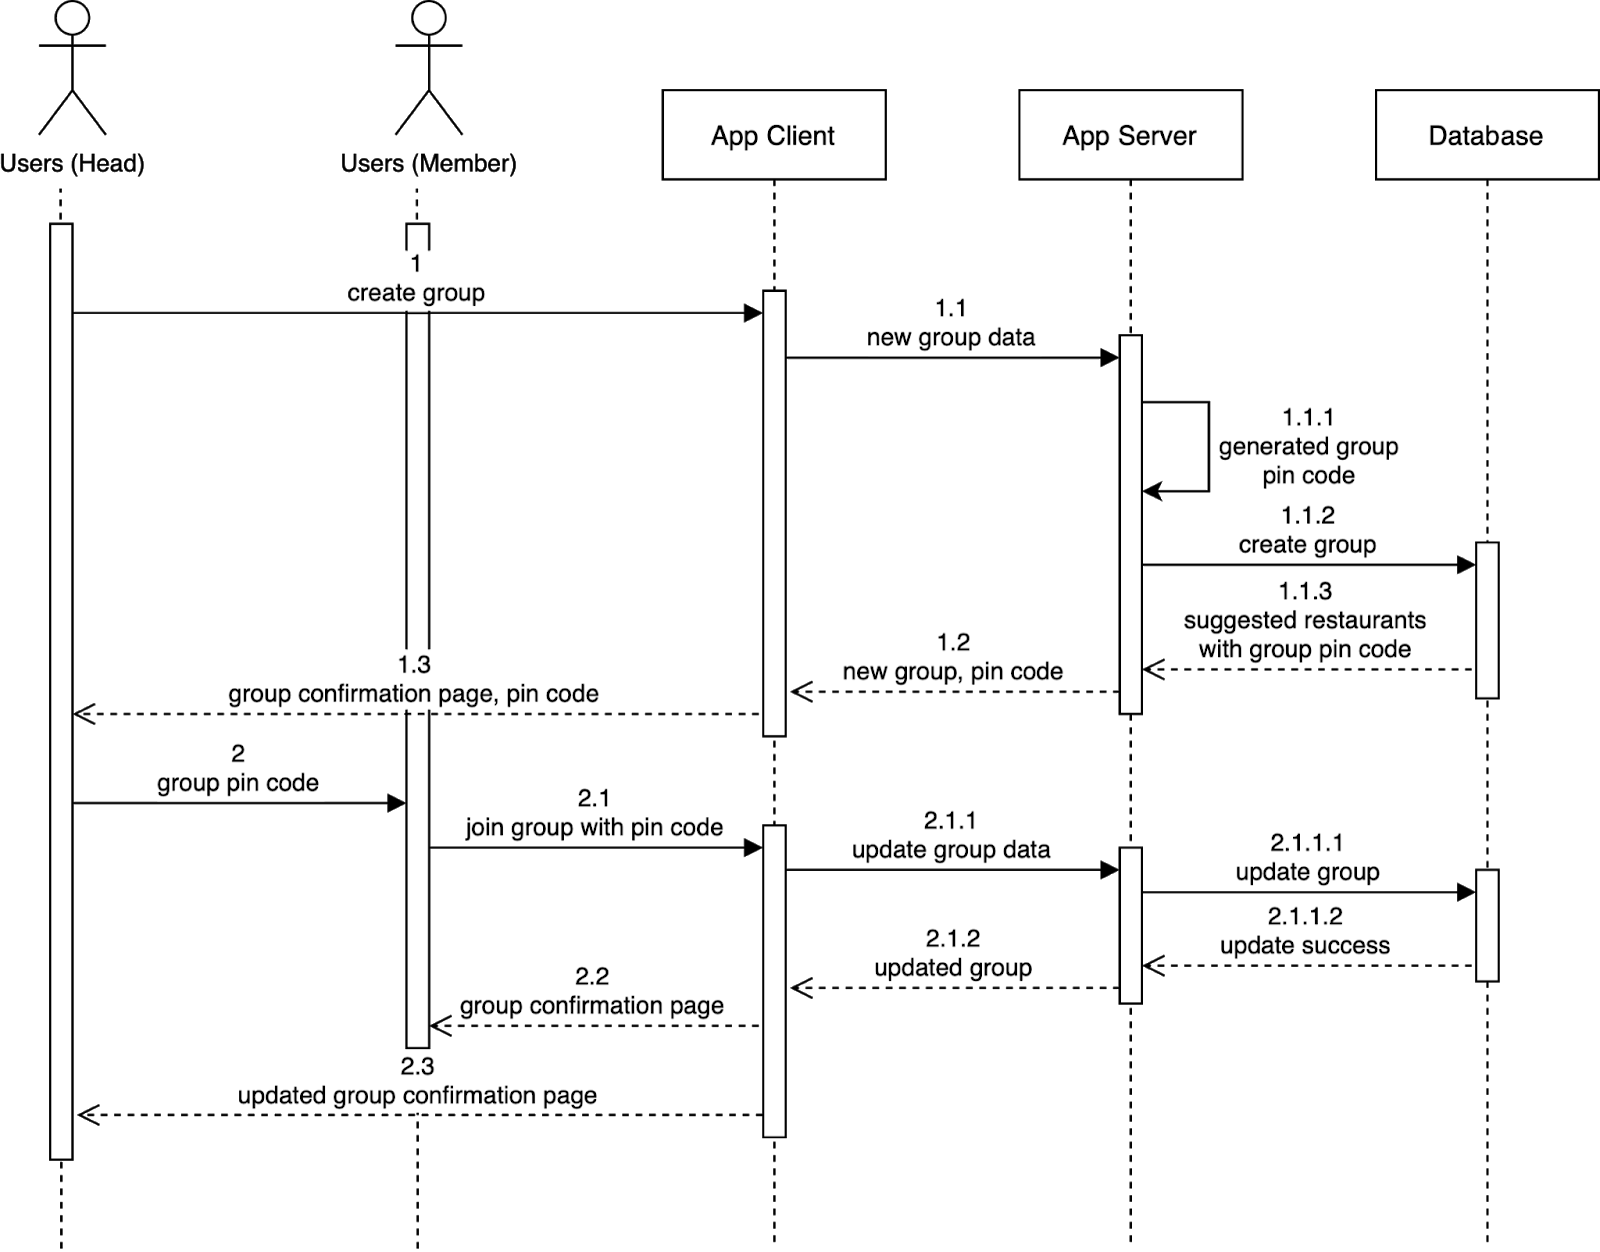
\includegraphics[width=400pt]{./images/3seqdiagram_creategroup.png}
\caption{Create Group Sequence Diagram}\label{fig:3seqdiagram_creategroup}
\end{figure}

\textbf{Scenario}: A group of 2 people wants to create a new eating group by the first user creating a group and the other one joining the group.
\begin{enumerate}
\item The first member creates a group (1). App Client sends data to App Server (1.1). App Server generates a group pin code (1.1.1) and creates a new record in the database (1.1.2). Finally, the member will see a group confirmation page and a group pin code (1.3).
\item After the member has the group pin code, they can share it to other members (2). When other members join a group with a pin code (2.1), App Server will update the record in the database (2.1.1) and other members will see the same group confirmation page as the person who created a group (2.2). The group information of the first member will also be updated (2.3).
\end{enumerate}


\newpage

\subsubsection{Group Restaurant Recommendation}

\begin{figure}[!h]\centering
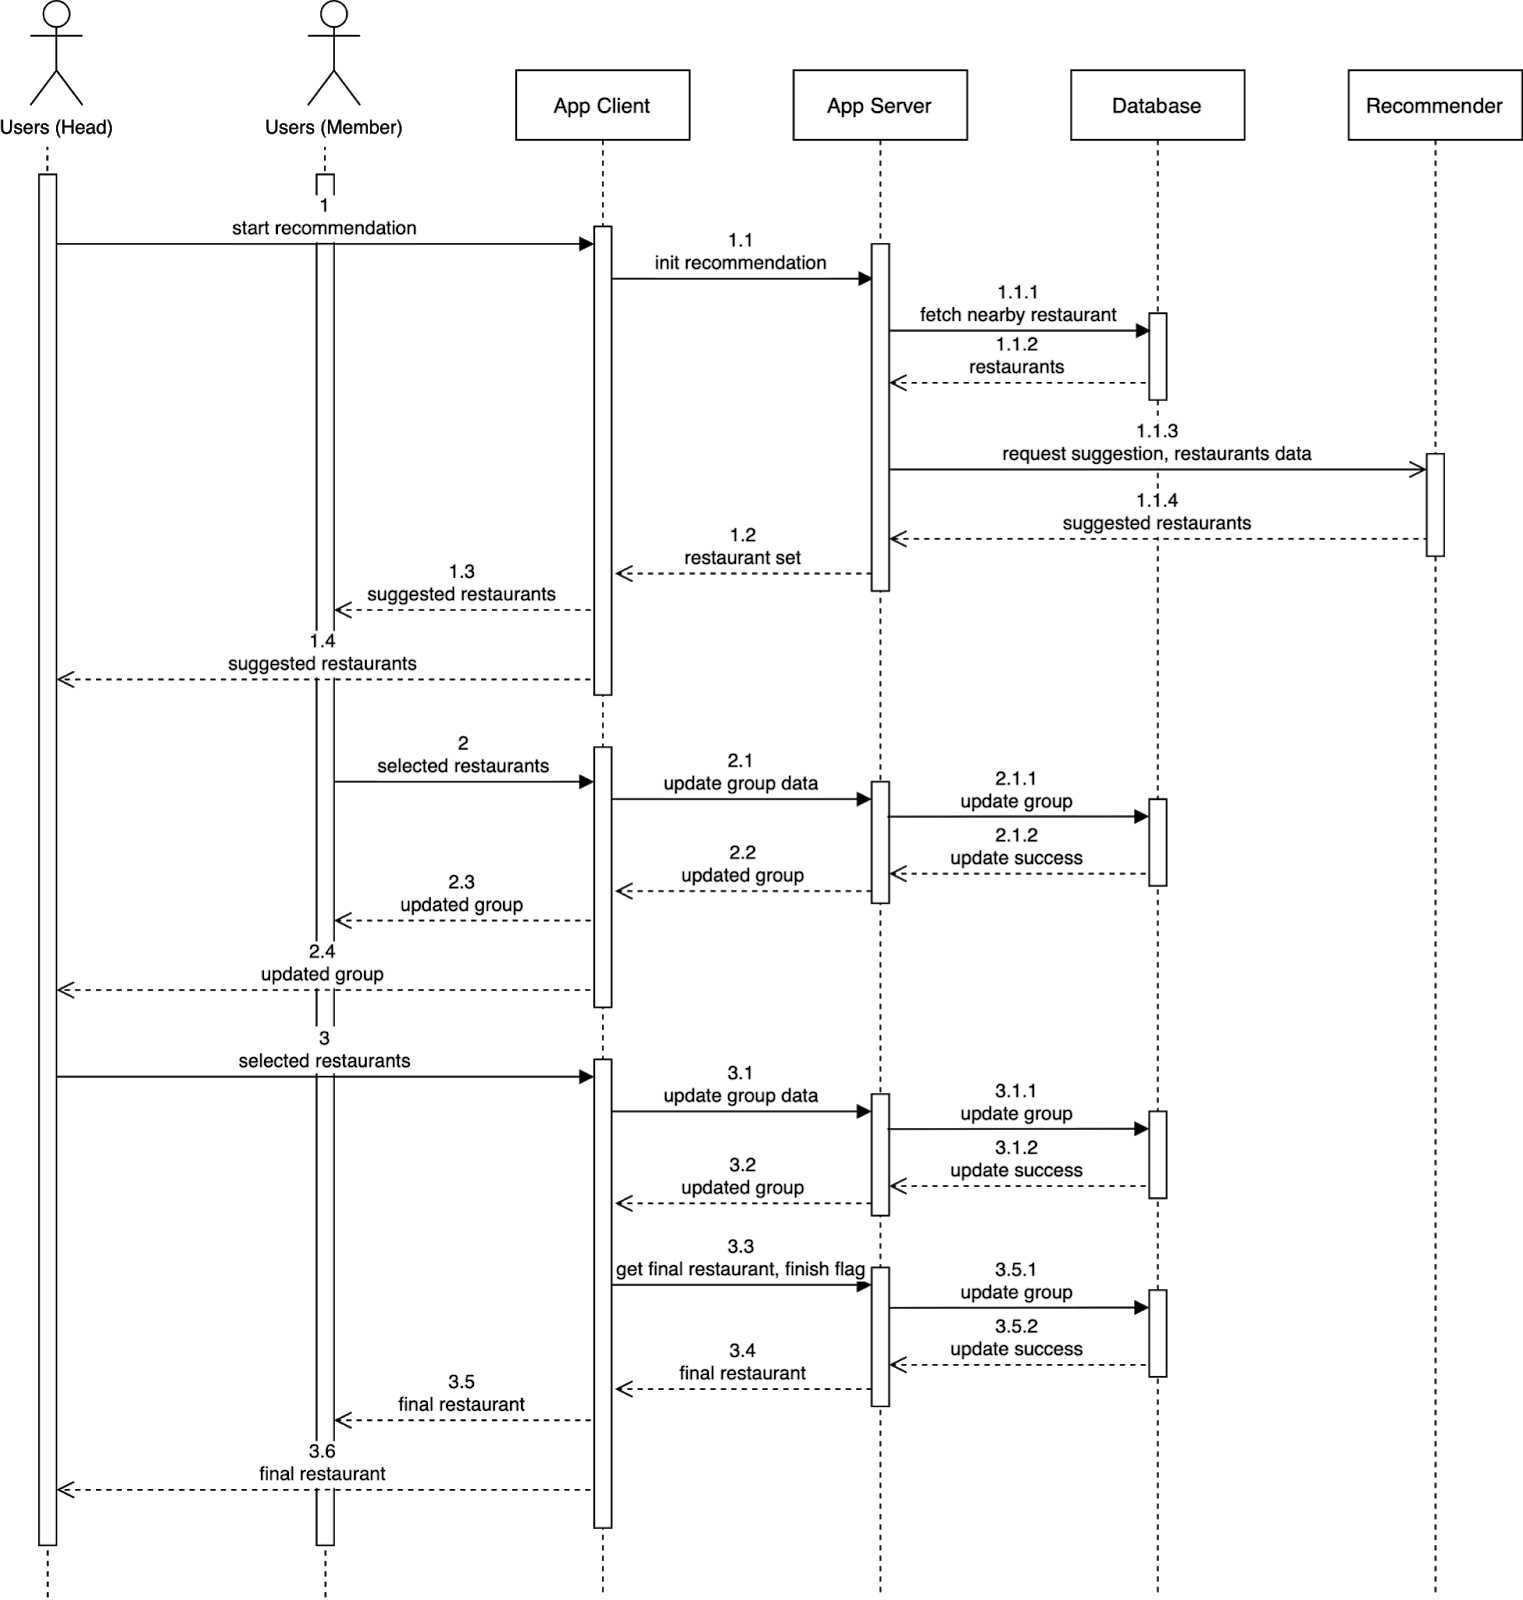
\includegraphics[width=400pt]{./images/3seqdiagram_grouprec.png}
\caption{Create Group Sequence Diagram}\label{fig:3seqdiagram_grouprec}
\end{figure}

\newpage
\textbf{Scenario}: A group of 2 people wants to have a restaurant recommendation for their group and they already have a group created.
\begin{enumerate}
\item When a head of the group which is the first member who created the group chooses to start a recommendation (1), App Client will request a new group recommendation to App Server (1.1). After that App Server and Recommender will generate a suggestion which has the same process as the individual recommendation (1.1.1 to 1.1.4). Note that Recommender can handle multiple users in the recommendation. Finally, the same suggested restaurant set will be shown to all members (1.3 and 1.4).
\item The first member finishes selecting their restaurant by their preference (2). App Server will update a group data (2.1) and both of the members will receive the update group data (2.3 and 2.4). However, the recommendation is not completed yet, it needs to wait for the other member to finish selecting the restaurants.
\item The second member finishes selecting the restaurants (3). App Server will update a group data again (3.1). In this time, App Client detects that every member has finished selecting the restaurant, so it will send a group finalization request with a finish flag (3.3). App Server will finalize the final restaurant to the group (3.3.1) and update the group data again (3.3.2). Finally, the final restaurant will be shown to every member (3.5 and 3.6) and the recommendation will be completed.
\end{enumerate}




\section{User Interface Design}
This section presents the user interface design of the restaurant recommendation system which designs in the Figma application.

The user interface of our web application includes login, registration, individual restaurant recommendation, group restaurant recommendation, and users’ profile as follows.

\newpage
\subsection{Login Page}
\begin{figure}[!h]\centering
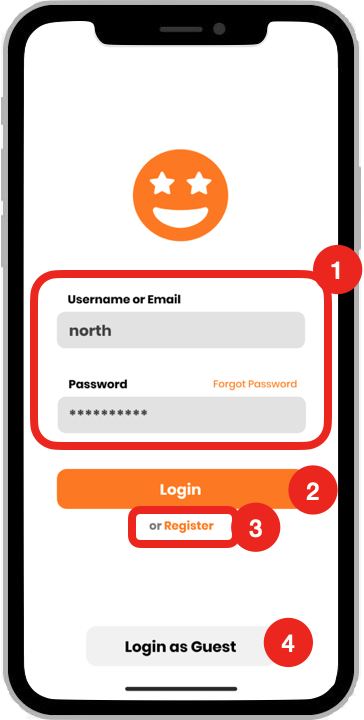
\includegraphics[height=300pt]{./images/3ui_StartPageUserInterfaceDesign.png}
\caption{Start Page User Interface Design}\label{fig:3ui_StartPageUserInterfaceDesign}
\end{figure}
\begin{enumerate}
\item Username and password input fields
\item Login button to confirm the input fields
\item Register button, it links to the registration page
\item Login as Guest for users who do not want an account but want to start using our system right away.
\end{enumerate}
When users open the application, the login page will appear first if they did not login yet. They need to input their username and password in the fields (1) then They can tap the “Login” button (2) to log in. After login, they will see the home page (Figure 3.19). If they do not have an account, they can tap on the “Register” button (3) and they will see the registration page (Figure 3.17). However, they can choose to login without any account by tapping on the “Login as Guest” button (4) and the system will directly bring them to the home page (Figure 3.19).
\newpage
\subsection{Registration Page}
\begin{figure}[!h]\centering
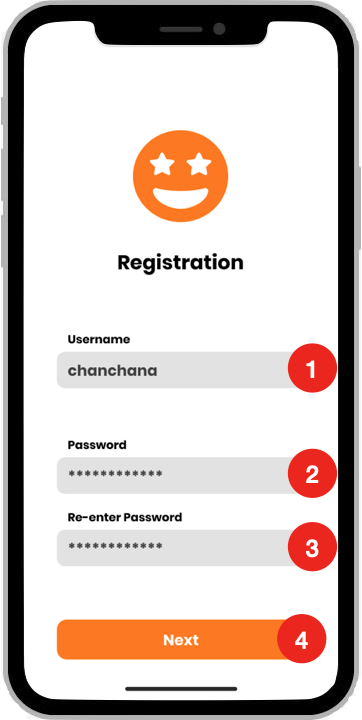
\includegraphics[height=300pt]{./images/3ui_RegistrationPageUserInterfaceDesign.png}
\caption{Registration Page User Interface Design}\label{fig:3ui_RegistrationPageUserInterfaceDesign}
\end{figure}
\begin{enumerate}
\item New username field
\item New password field
\item Re-enter the password field, it needs to be matched with the password field
\item Next button, links to a general information setup page
\end{enumerate}
If users choose to register, the registration page will appear and ask users to input a new username, password, and re-enter the password (1), (2), (3) respectively. If the input username is invalid or already taken, the system will alert users and let them choose a new username. If the password field and re-enter password field are mismatched, the system will also alert and tell users to input their password and re-enter password fields again. After all of the information in the fields is valid and users tap on the “Next” button (4), they will proceed to the next step which is the profile setting step stated in~\ref{fig:3ui_ProfileSetupPageUserInterfaceDesign}.
\newpage
\begin{figure}[!h]\centering
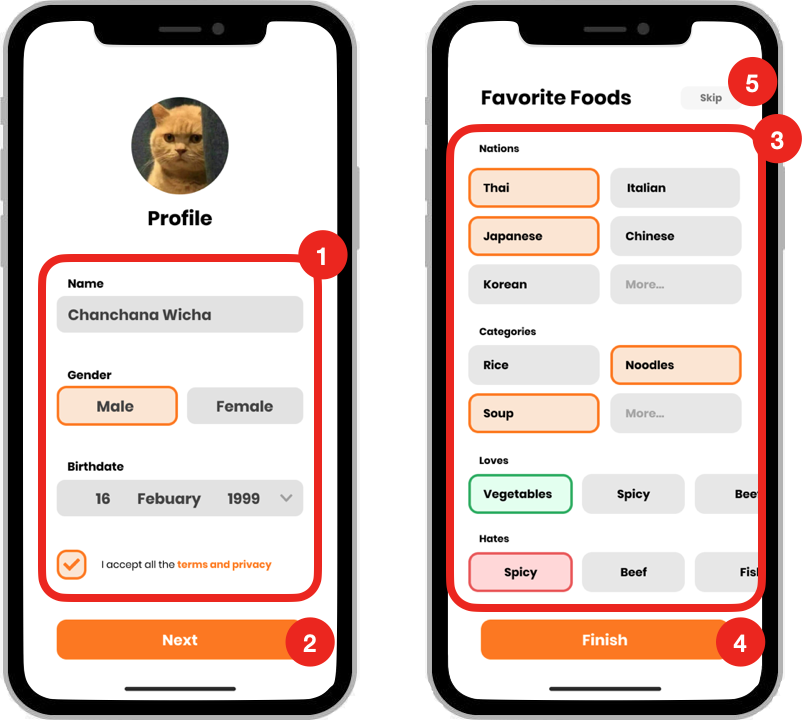
\includegraphics[height=300pt]{./images/3ui_ProfileSetupPageUserInterfaceDesign.png}
\caption{Profile Setup Page User Interface Design}\label{fig:3ui_ProfileSetupPageUserInterfaceDesign}
\end{figure}
\begin{enumerate}
\item General information form
\item Next button, will proceed users to the food preference setup step
\item Food preference form, let users choose their food preference in each category.
\item Finish button, to complete the form and the registration.
\item Skip button, lets users skip the food preference setup process.
\end{enumerate}
After users input the valid username and password, the next step is user profile setup. This process consists of 2 steps which are general information setup and food preferences information setup. The first one on the left of~\ref{fig:3ui_ProfileSetupPageUserInterfaceDesign} is a general information setup step. Users are required to fill in all the information in the form and accept the terms and privacy (1) then they can proceed to the next step by tapping the “Next” button (2). For the second step, preferences information set up, they will see many available categories of food. They can choose their food preferences in the form (3) and tap on “Finish” to complete the registration. However, if they do not want to set their preferences yet, they can tap on the “Skip” button (5) to skip the preferences setup process. After the registration is completed, they will see the home page (Figure 3.19) and start using our system.
\newpage
\subsection{Individual Restaurant Recommendation Page}
\begin{figure}[!h]\centering
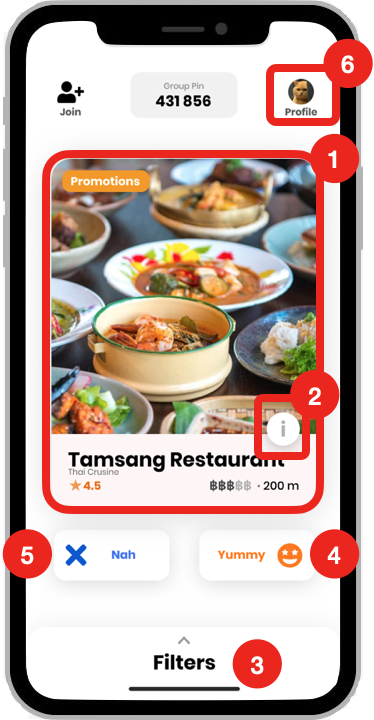
\includegraphics[height=300pt]{./images/3ui_HomePageUserInterfaceDesign.png}
\caption{Home Page User Interface Design}\label{fig:3ui_HomePageUserInterfaceDesign}
\end{figure}
\begin{enumerate}
\item Restaurant card, it shows the general information about a restaurant.
\item “i” button, when tapped, more information will be shown.
\item 
\item Like button, tapped once users are satisfied with the restaurant
\item Dislike button, if users are not satisfied with the restaurant, they can tap this button to see the next suggestion.
\item Profile button, links to the profile page.
\end{enumerate}
After users logged in or registered, they will see the home page. By entering the home page, the system will automatically start recommending some restaurants to users. Users will see the information of each suggested restaurant (1). They can also see some more information about each restaurant by tapping the “i” icon (2). They can filter the suggested restaurants by tapping the “Filters” button (3) and the filter window will appear (Figure 3.20). If they are satisfied with the suggested restaurant, they can tap on the “Yummy” button (4) or swipe the restaurant card to the right, and then the success page will appear (Figure 3.21). Otherwise, if they are not satisfied with that restaurant, they can tap on the “Nah” button (5) or swipe the restaurant card to the left, and then the system will show the next suggested restaurant to users and let them consider it again. Users can see their profile by tapping the profile picture button (6) and the profile management page will appear (Figure 3.25).
\begin{figure}[!h]\centering
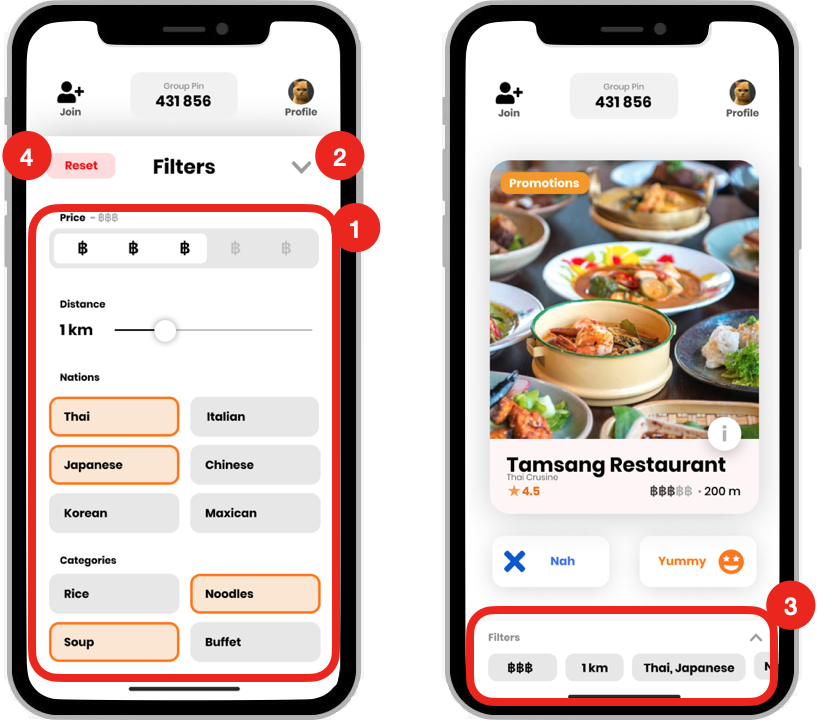
\includegraphics[height=300pt]{./images/3ui_FilterWindowUserInterfaceDesign.png}
\caption{Filter Window User Interface Design}\label{fig:3ui_FilterWindowUserInterfaceDesign}
\end{figure}
\begin{enumerate}
\item Filtering options.
\item Arrow button, will apply current filtering and close the filter window.
\item Filter button with applied filter tags, users can open the filter window again by tapping this button.
\item Reset button, will remove all the applied filters.
\end{enumerate}
After users tap on the “Filter” button on the home page (number 3 on~\ref{fig:3ui_HomePageUserInterfaceDesign}), the filter window will appear. Users can filter restaurants by choosing the available options that appear on the filter window (1). After finishing choosing the filtering option, they can tap on the arrow icon (2) to apply the filter and the filter window will be minimized. They can see the applied filters at the bottom of the screen (3). They can change their filtering by tapping on the bottom bar (3) to bring the filter window up again. They can tap on the “Reset” button (4) to remove all of the applied filters. After applying any filters, the system will suggest the restaurant that matches its filtering condition.
\newpage
\begin{figure}[!h]\centering
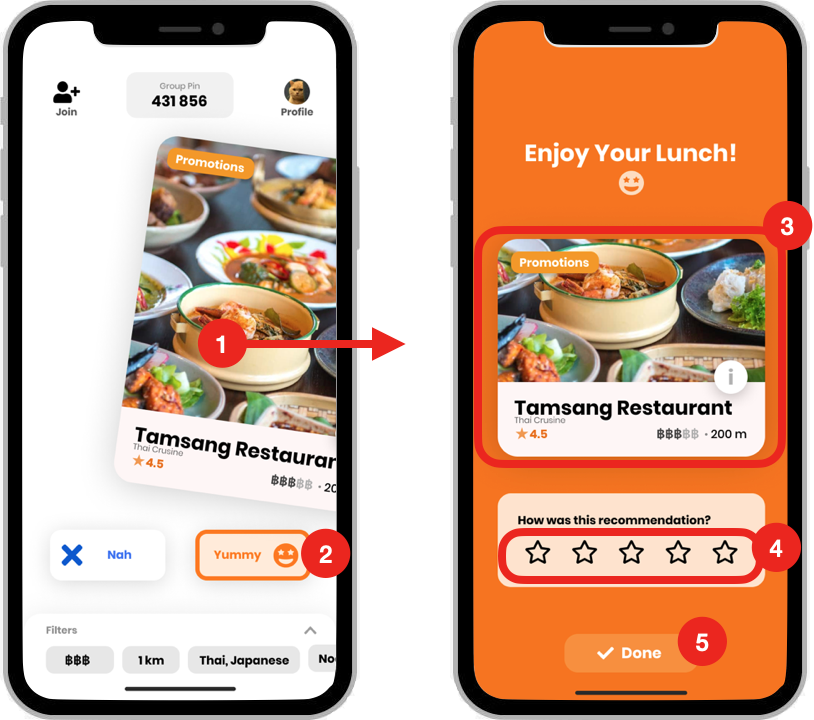
\includegraphics[height=300pt]{./images/3ui_RecommendationSuccessPageUserInterfaceDesign.png}
\caption{Recommendation Success Page User Interface Design}\label{fig:3ui_RecommendationSuccessPageUserInterfaceDesign}
\end{figure}
\begin{enumerate}
\item Swipe right for the satisfying restaurant.
\item Like button which works the same as the swipe right.
\item Restaurant card showing general information about the liked restaurant.
\item Recommendation rating, let users rate satisfaction with their current recommendation.
\end{enumerate}
On the home page which users see the suggested restaurant, if users are satisfied with the suggested restaurant, they can swipe right (1) or tap on the “Yummy” button (2). After that, the recommendation success page will appear (the right picture in~\ref{fig:3ui_RecommendationSuccessPageUserInterfaceDesign}). On the success page, users can see the restaurant information in the center of the screen (3). They can give a rating score for the recommendation from 1 star to 5 stars (4). After they are done seeing the information, they can tap on the “Done” button (5) to close the success page and they will see the home page (Figure 3.19) again.
\newpage
\subsection{Group Restaurant Recommendation Page}
\begin{figure}[!h]\centering
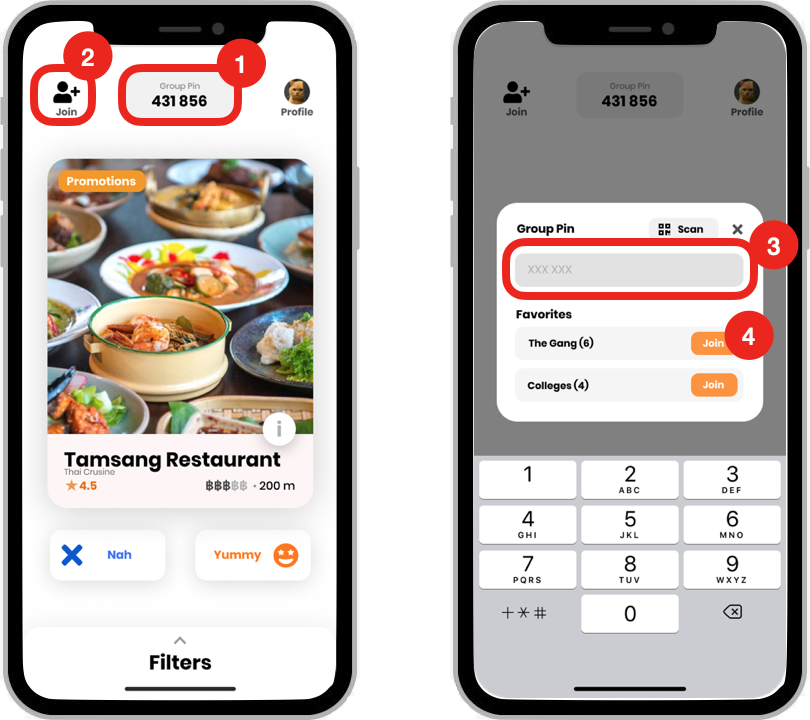
\includegraphics[height=300pt]{./images/3ui_GroupJoiningUserInterfaceDesign.png}
\caption{Group Joining User Interface Design}\label{fig:3ui_GroupJoiningUserInterfaceDesign}
\end{figure}
\begin{enumerate}
\item Group pin code which other members used for joining the group.
\item Join button, it will bring up the joining dialog
\item Group pin code input field, let users input the group pin code.
\item Join button which lets users join their existing group without input the group pin code again.
\end{enumerate}
In the following section, we will walk through the group recommendation process. On the home page (the left picture in~\ref{fig:3ui_GroupJoiningUserInterfaceDesign}), it will show the group pin on the top of the screen (1). To start the group recommendation, the user has to share this pin code with other members in the group and this will make the pin code owner be the head of the group. Other members can join the group by tapping on the “Join” button (2) and the joining dialog will appear (the right picture in~\ref{fig:3ui_GroupJoiningUserInterfaceDesign}). In the joining dialog, other members can input the pin that appeared on the group head’s device (1). Moreover, users can join the previously joined group, which will be shown as favorites. They can directly join their favorite group by tapping the “Join” button (4) in the group they want to join without input the pin code again. After someone joins the group the group recommendation will be initialized and all members that joined the group will see the group confirmation page next (Figure 3.23).
\newpage
\begin{figure}[!h]\centering
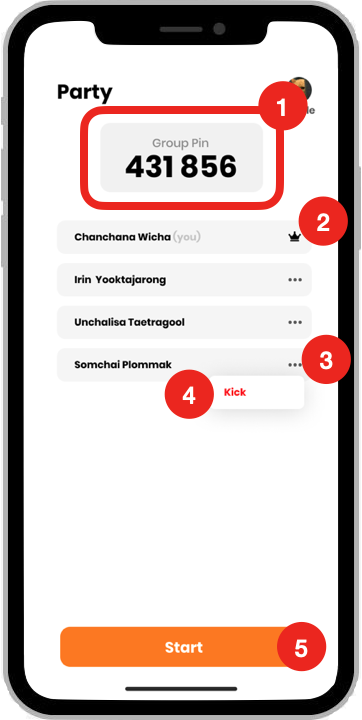
\includegraphics[height=300pt]{./images/3ui_GroupConfirmationPageUserInterfaceDesign.png}
\caption{Group Confirmation Page User Interface Design}\label{fig:3ui_GroupConfirmationPageUserInterfaceDesign}
\end{figure}
\begin{enumerate}
\item Group pin code which other members used for joining the group.
\item Crown icon indicates who is the head of this group
\item 3 dots icon for more action on each member in the group.
\item Kick button, it let the head remove some members from the group.
\end{enumerate}
After someone joins the group, all joined members will see this group confirmation page. On the top, there is a group pin code that the members in the group can share with other people if they want to join this eating group. The head of the group will have a crown icon (2) and they can manage the members in the group. If the head wants to remove some of the members, they can do it by tapping the 3 dots icon (3) followed by tapping the “Kick” button, after that the kicked member will no longer be in the party. When all members are joined and ready, the head will tap on the “Start” button to begin the group recommendation.
\newpage
\begin{figure}[!h]\centering
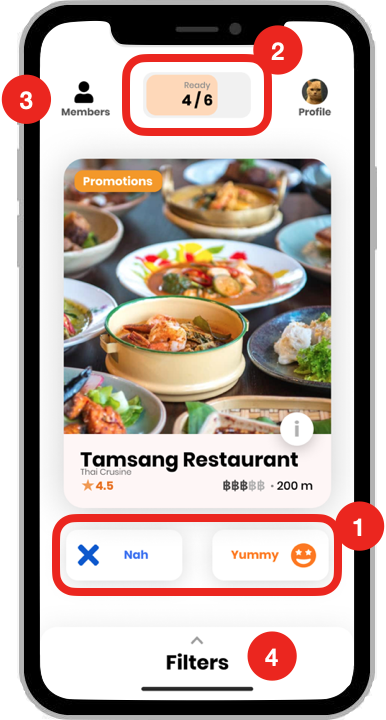
\includegraphics[height=300pt]{./images/3ui_GroupRecommendationPageUserInterfaceDesign.png}
\caption{Group Recommendation Page User Interface Design}\label{fig:3ui_GroupRecommendationPageUserInterfaceDesign}
\end{figure}
\begin{enumerate}
\item Like or dislike area for choosing the restaurant.
\item Progress bar indicates the progress of the group decision.
\item Members button, will bring up the members dialog which shows all members.
\item Filter button for setting the filters for restaurants.
\end{enumerate}
After the group has been created and confirmed, the group recommendation will begin. All members will see the same suggested set of restaurants. Each member will choose whether they like or not but tapping “Yummy” and “Nah” or swiping (1) is the same as in individual recommendation. The group recommendation will be finished after all members like the same restaurant. The top bar (2) indicates the highest number of members that agree on the same restaurant, when it is full, it means everybody agrees on the same restaurant and the recommendation is finished. Users can see the members by tapping the “Member” button (3). Users still can set the filter by tapping the “Filter” button (4) but this time the filters will be applied to every member in the group.
\newpage
\subsection{Profile Page}
\begin{figure}[!h]\centering
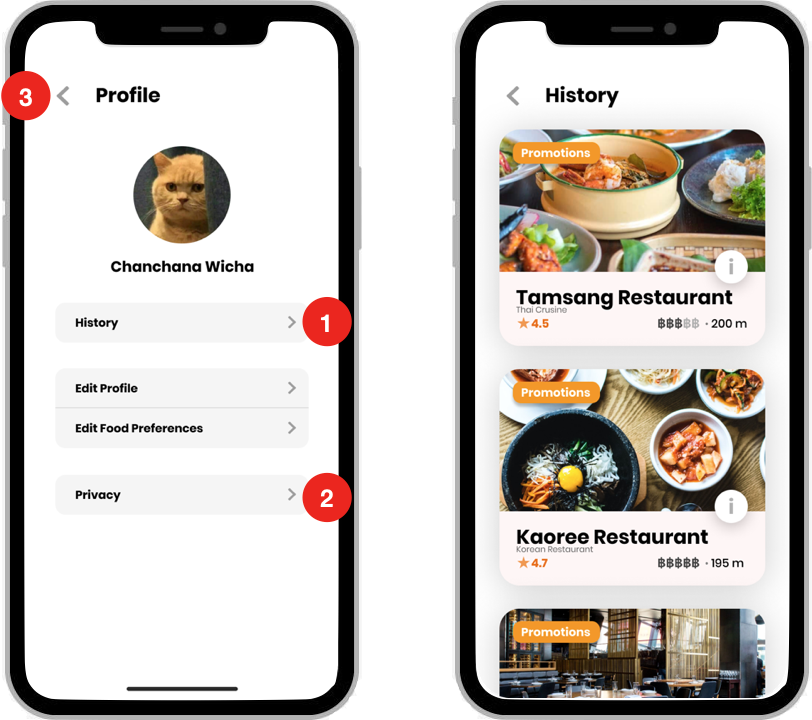
\includegraphics[height=300pt]{./images/3ui_ProfileManagementPageUserInterfaceDesign.png}
\caption{Profile Management Page User Interface Design}\label{fig:3ui_ProfileManagementPageUserInterfaceDesign}
\end{figure}
\begin{enumerate}
\item History button, it links to the history page (the right picture in Figure 3.25)
\item Privacy button, it let users change their password and their privacy setting.
\item Back button which brings users back to their home page.
\end{enumerate}
After users choose to view their profile (number 6 in~\ref{fig:3ui_HomePageUserInterfaceDesign}), they will see the left picture in~\ref{fig:3ui_ProfileManagementPageUserInterfaceDesign}. They can choose to view their selected restaurant history by tapping the “History” button (1) and a list of selected restaurants will be shown (the right picture of~\ref{fig:3ui_ProfileManagementPageUserInterfaceDesign}). They can also choose to edit their profile such as their name, gender, or birthdate or choose to edit their food preferences. They can reset their password and set the privacy setting under the “Privacy” section (2). They can go back to the main screen by tapping the arrow icon (3).


\section{Database Structure}
In this section, we explain our database structure in the Database component. Our database stores all information for our system as a NoSQL database. Then, we discuss the database collection’s name and description, the schema of each collection, and database indexing.

\newpage
\subsection{Collections}
\begin{table}[!h]
\caption{Database Collection and Description}\label{tbl:3DatabaseCollectionandDescription}
\begin{tabularx}{\textwidth}{l|X} \hline\hline
Collection Name & Description \\ \hline\hline
restaurants & Restaurant information including name, address, photo URL, etc., restaurant profile. \\ \hline
users & User information including authentication information, general information such as name, gender, age, and food preference information. \\ \hline
recommendations & Information for each recommendation session. This collection includes all of the interaction histories from the user in each recommendation session. \\ \hline
categories & Information about restaurant categories. We keep the categories separated with restaurant collection to reduce the redundancy. \\ \hline
favorites & Keep the information about the favorite list of restaurants for each user. \\ \hline\hline
\end{tabularx}
\end{table}

Table ~\ref{tbl:3DatabaseCollectionandDescription} shows us all collections in our NoSQL database, their collection’s name, and their description. Our database contains mainly 5 collections including restaurants, users, recommendations, categories, and favorites.

\subsection{Schema}

Although NoSQL does not have a fixed database schema, by using Mongoose as a MongoDB database connection framework, it provides some primary schema for data creating and reading facilitation. Having Mongoose’s schema can help us manage a uniform data format with easy schema migration. However, inserting data with a different format from Mongoose’s schema does not break the process and no part of the data will be discarded. In this section, we will show some mandatory fields for each collection.


\begin{table}[!h]
\caption{Restaurant Schema}\label{tbl:3RestaurantSchema}
\begin{tabularx}{\textwidth}{l|l|X} \hline\hline
Key Name & Type & Description \\ \hline\hline
name & String & Name of the restaurant \\ \hline
profile.categories & Array of ObjectId & Restaurant categories such as Thai, Korean, Fast Food. This field references category collection using their category id. \\ \hline
profile.price\_range & Number & The price range of the restaurant, from 1-4. \\ \hline
profile.rating & Number & Facebook users’ rating of the restaurant. From 1 to 5 stars. \\ \hline
profile.likes & Number & The number of users that liked the restaurant’s Facebook page. \\ \hline
address & String & One line address string of the restaurant. \\ \hline
location.coordinates & Array of Numbers & Coordinate of the restaurant in form of [longitude, latitude] \\ \hline
link & String & URL link to their Facebook page. \\ \hline\hline
\end{tabularx}
\end{table}

\begin{table}[!h]
\caption{User Schema}\label{tbl:3UserSchema}
\begin{tabularx}{\textwidth}{l|l|X} \hline\hline
Key Name & Type & Description \\ \hline\hline
authentication & Object & Authentication token object for user login. \\ \hline
username & String & Username of the user. \\ \hline
password & String & Encrypted password of the user. \\ \hline
profile.gender & String & Gender of the user. \\ \hline
profile.birthdate & Date & Birthdate of the user. \\ \hline
profile.preference & Object & Food preferences of users. \\ \hline\hline
\end{tabularx}
\end{table}

\begin{table}[!h]
\caption{Recommendation Schema}\label{tbl:3RecommendationSchema}
\begin{tabularx}{\textwidth}{l|l|X} \hline\hline
Key Name & Type & Description \\ \hline\hline
users & Array of ObjectId & Users that request the recommendation. This field references user collection using their user id. \\ \hline
histories & Array of Object & User interaction history in each recommendation session. \\ \hline
histories.restaurant & ObjectId & Interacted restaurant. This field references restaurant collection using their restaurant id. \\ \hline
histories.is\_love & Boolean & Whether users select go or not go to the interacted restaurant. \\ \hline
histories.timestamp & Date & The timestamp of each interaction history. \\ \hline
location.coordinate & Array of Numbers & The location that this recommendation session occurs in the form of [longitude, latitude]. \\ \hline\hline
\end{tabularx}
\end{table}

\begin{table}[!h]
\caption{Category Schema}\label{tbl:3CategorySchema}
\begin{tabularx}{\textwidth}{l|l|X} \hline\hline
Key Name & Type & Description \\ \hline\hline
name & String & Name of the category eg. Thai Restaurant, Korean Restaurant, or Fast Food Restaurant. \\ \hline
is\_common & Boolean & Whether this category is a common category. \\ \hline\hline
\end{tabularx}
\end{table}

\begin{table}[!h]
\caption{Favorite Schema}\label{tbl:3FavoriteSchema}
\begin{tabularx}{\textwidth}{l|l|X} \hline\hline
Key Name & Type & Description \\ \hline\hline
user & ObjectId & User of the current record. \\ \hline
restaurants & Array of & List of their favorite restaurants. \\ \hline\hline
\end{tabularx}
\end{table}

Note that we need to keep a category collection separated from restaurant information because some of the collected restaurant data may have a different name but same id or different id with the same name so we want to keep this information correctly and easily maintained later.


\subsection{Indexing}

With database indexing, we can query the data faster by storing additional information about data. Every collection has an indexed id so that we can query the data from their id faster. However, we also set more indexing on 2 collections which are restaurants and users.

\begin{figure}[!h]\centering
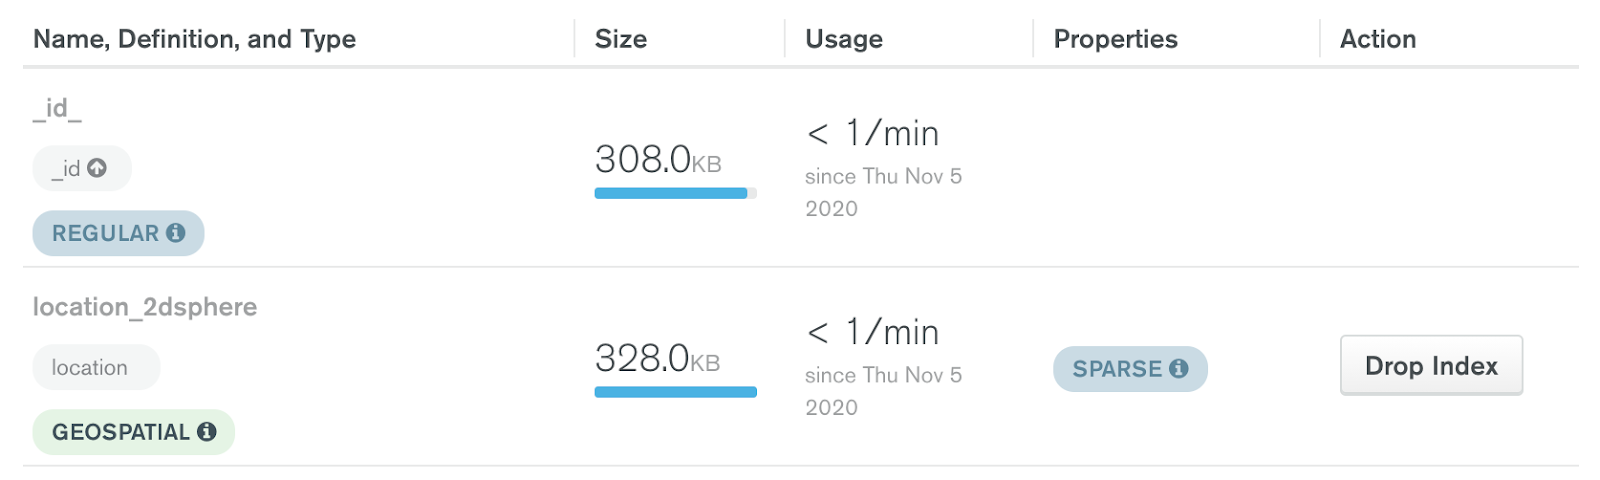
\includegraphics[width=400pt]{./images/3db_RestaurantCollectionsIndexes.png}
\caption{Restaurant Collection’s Indexes}\label{fig:3db_RestaurantCollectionsIndexes}
\end{figure}

From~\ref{fig:3db_RestaurantCollectionsIndexes}, we can see that the restaurant collection has one more index which is the location index. This index is used for query restaurants by a distance of 2 coordinates.
\begin{figure}[!h]\centering
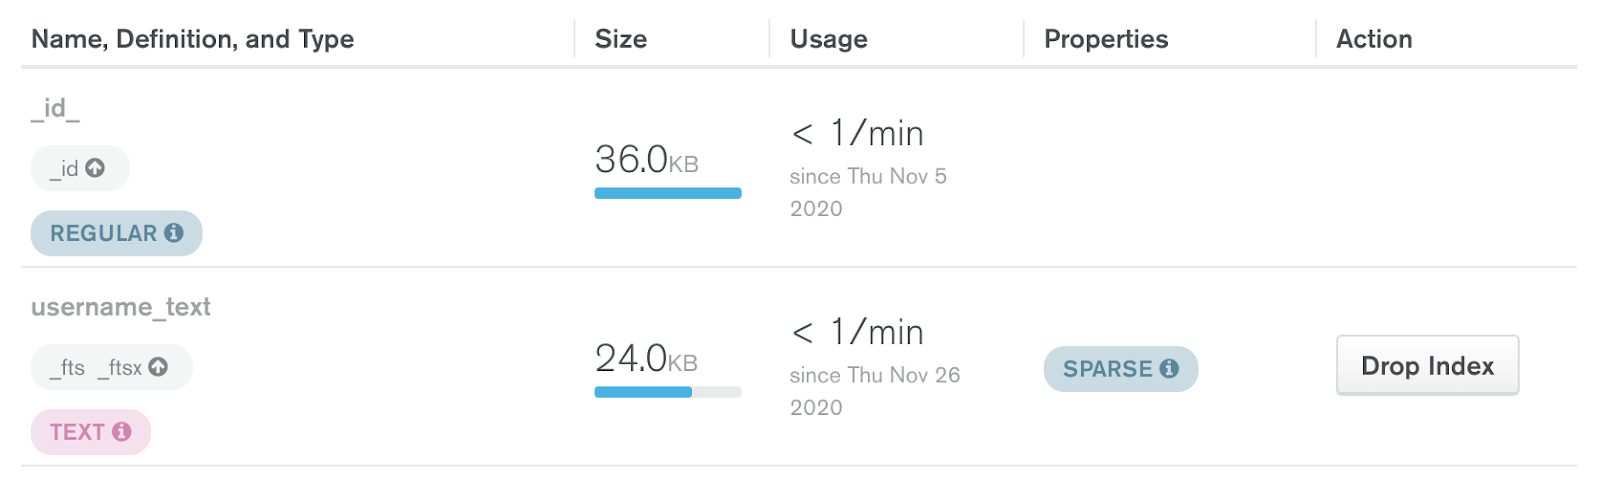
\includegraphics[width=400pt]{./images/3db_UserCollectionsIndexes.png}
\caption{User Collection’s Indexes}\label{fig:3db_UserCollectionsIndexes}
\end{figure}

From~\ref{fig:3db_UserCollectionsIndexes}, we can see that the user collection has one more index which is the username index. This index is used for query users by username. It also helps when checking the username’s availability. The username index also applies to other collections that require finding  the record by the username which is the favorite collection.


\section{Restaurant Recommendation Algorithm}
%TODO

\section{Production Testing Plan}

\subsection{Production Deployment}

We will deploy our components that need to listen to requests and send requests to other components which are App Client, App Server, Recommender, and Database. App Client, App Server, and Recommender will be deployed on Google Cloud App Engine since the deployment service is flexible for multiple programming languages and supports auto scalability. Database will be deployed on MongoDB Atlas which is an official cloud deployment service for MongoDB databases. Both Google Cloud App Engine and MongoDB Atlas provide an interactive dashboard for monitoring the performance.

\subsection{User Evaluation}

We will test our application and gather feedback from 20 people. We will collect the data about overall satisfaction, usability, user experience, and improvement suggestions. After the data has been collected, we will analyze and evaluate the application.

\subsection{Application Evaluation}

The performance of main components, App Client, App Server, and Recommender, will be evaluated by monitoring the response latency and doing load tests. The production application performance metrics can also be retrieved by the Google Cloud App Engine dashboard.



\section{Recommender Systems}

%\url{http://www.cpe.kmutt.ac.th}
%Explain theory, algorithms, protocols, or existing research works and tools related to your work. \cite{bworld}

\begin{table}[!h]
\caption{test table method1}\label{tbl:method1}
\begin{tabular}{c|c|l|rr} \hline\hline
Center & Center & left aligned & Right & Right aligned \\ \hline\hline
Center & Center & left aligned & Right & Right aligned \\ \hline
Center & Center & left aligned & Right & Right aligned \\ 
Center & Center & left aligned & Right & Right aligned \\ \hline
Center & Center & left aligned & Right & Right aligned \\ \hline\hline
\end{tabular}
\end{table}


\section{Text Processing Algorithms}
\subsection{Algorithm I}

% Can define this in the preamble..
You can place the figure and refer to it as Figure~\ref{fig:model2}.
The figure and table numbering will be run and updated automatically when you add/remove tables/figures from the document.

\begin{figure}[!h]\centering
\setlength{\fboxrule}{0.2mm} % can define this in the preamble
\setlength{\fboxsep}{1cm}
\fbox{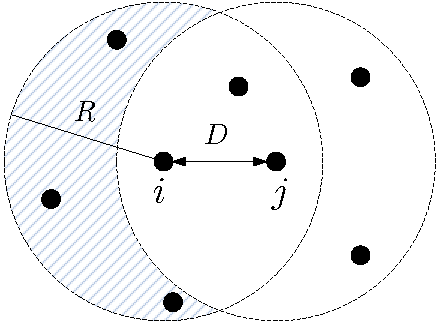
\includegraphics[width=5cm]{./model2.pdf}}
\caption{The network model}\label{fig:model2}
\end{figure}

 
\subsection{Algorithm II}
Add more subsections as you want.

\subsubsection{Algorithm SUB}
Add more subsections as you want.


\section{Development Tools}

%%%%%%%%%%%%%%%%%%%%%%%%%%%%%%%%%%%%%%%%%%%%%%%%%%%%%55
%%%%%%%%%%%%%%%%%%%%%%%%%%%%%%%%%%%%%%%%%%%%%%%%%%%%%
%%%%%%%%%%%%%%%%%%%%%%%%%%%%%%%%%%%%%%%%%%%%%%%%%%%%%
\chapter{Proposed Work}

Explain the design (how you plan to implement your work) of your project. Adjust the section titles below to suit the types of your work. Detailed physical design like circuits and source codes should be placed in the appendix.

\section{System Architecture}

\begin{table}[!h]
\centering
\caption{test table x1}\label{tbl:symbols}
\begin{tabular}{@{}p{0.07\textwidth}|p{0.7\textwidth}p{0.1\textwidth}}\hline
\multicolumn{2}{l}{\textbf{SYMBOL}}  & \textbf{UNIT} \\ \hline 
$\alpha$ & Test variable\hfill & m$^2$ \\
$\lambda$ & Interarrival rate\hfill &  jobs/second\\
$\mu$ & Service rate\hfill & jobs/second \\ \hline
\end{tabular}
%\begin{tabular}{c|c} \hline
% $\alpha$ & $\beta$ \\ \hline
% $\delta$ & $\mu$ \\ \hline
%\end{tabular}
\end{table}

\section{System Specifications and Requirements}

\section{Hardware Module 1}
\subsection{Component 1}
\subsection{Logical Circuit Diagram}

\section{Hardware Module 2}
\subsection{Component 1}
\subsection{Component 2}

\section{Path Finding Algorithm}

\section{Database Design}

\section{GUI Design}



%%%%%%%%%%%%%%%%%%%%%%%%%%%%%%%%%%%%%%%%%%%%%%%%%%%%%%%%%%%%%%
%%%%%%%%%%%%%%%%%%%% Experiments %%%%%%%%%%%%%%%%%%%%%%%%%%%%%
%%%%%%%%%%%%%%%%%%%%%%%%%%%%%%%%%%%%%%%%%%%%%%%%%%%%%%%%%%%%%%%
\chapter{Implementation Results}

You can title this chapter as \textbf{Preliminary Results} or \textbf{Work Progress} for the progress reports. Present implementation or experimental results here and discuss them.

%%%%%%%%%%%%%%%%%%%%%%%%%%%%%%%%%%%%%%%%%%%%%%%%%%%%%%%%%%%%%%%
%%%%%%%%%%%%%%%%%%%% Conclusions %%%%%%%%%%%%%%%%%%%%%%%%%%%%%
%%%%%%%%%%%%%%%%%%%%%%%%%%%%%%%%%%%%%%%%%%%%%%%%%%%%%%%%%%%%%%%
\chapter{Conclusions}

This chapter is optional for proposal and progress reports but 
is required for the final report.\cite{shen04}

\section{Problems and Solutions}
State your problems and how you fixed them.

\section{Future Works}
What could be done in the future to make your projects better.

%%%%%%%%%%%%%%%%%%%%%%%%%%%%%%%%%%%%%%%%%%%%%%%%%%%%%%%%%%%%%%%
%%%%%%%%%%%%%%%%%%%% Bibliography %%%%%%%%%%%%%%%%%%%%%%%%%%%%%
%%%%%%%%%%%%%%%%%%%%%%%%%%%%%%%%%%%%%%%%%%%%%%%%%%%%%%%%%%%%%%%

%%%% Comment this in your report to show only references you have
%%%% cited. Otherwise, all the references below will be shown.
\nocite{*}
%% Use the kmutt.bst for bibtex bibliography style 
%% You must have cpe.bib and string.bib in your current directory.
%% You may go to file .bbl to manually edit the bib items.
\bibliographystyle{kmutt}
\bibliography{string,cpe}

%%%%%%%%%%%%%%%%%%%%%%%%%%%%%%%%%%%%%%%%%%%%%%%%%%%%%%%%%%%%%%%
%%%%%%%%%%%%%%%%%%%%%%%% Appendix %%%%%%%%%%%%%%%%%%%%%%%%%%%%%
%%%%%%%%%%%%%%%%%%%%%%%%%%%%%%%%%%%%%%%%%%%%%%%%%%%%%%%%%%%%%%%
\appendix{First appendix title}
\noindent{\large\bf Put appropriate topic here} \\

This is where you put hardware circuit diagrams, detailed experimental data in tables or source codes, etc.. \\ \bigskip



This appendix describes two static allocation methods for fGn (or fBm)
traffic. Here, $\lambda$ and $C$ are respectively the traffic arrival
rate and the service rate per dimensionless time step. Their unit are
converted to a physical time unit by multiplying the step size
$\Delta$. For a fBm self-similar traffic source,
Norros~\cite{norros95} provides its EB as
\begin{equation}\label{eq:norros}
  C = \lambda + (\kappa(H)\sqrt{-2\ln\epsilon})^{1/H}a^{1/(2H)}x^{-(1-H)/H}\lambda^{1/(2H)}
\end{equation}
where $\kappa(H) = H^H(1-H)^{(1-H)}$. Simplicity in the calculation is
the attractive feature of (\ref{eq:norros}).

The MVA technique developed in~\cite{kim01} so far provides the most
accurate estimation of the loss probability compared to previous
bandwidth allocation techniques according to simulation results.
Consider a discrete-time queueing system with constant service rate
$C$ and input process $\lambda_n$ with $\mathbb{E}\{\lambda_n\} =
\lambda$ and $\mathrm{Var}\{\lambda_n\} = \sigma^2$.  Define $X_n \equiv
\sum_{k=1}^n \lambda_k - Cn$.  The loss probability due to the MVA
approach is given by
\begin{equation}\label{eq:loss_mva}
  \varepsilon \approx \alpha e^{-m_x/2}
\end{equation}
where
\begin{equation}\label{eq:mx}
m_x = \min_{n \geq 0} \frac{((C-\lambda)n + B)^2}{\mathrm{Var}\{X_n\}} =
\frac{((C-\lambda)n^\ast + B)^2}{\mathrm{Var}\{X_{n^{\ast}}\}}
\end{equation} 
and 
\begin{equation}\label{eq:alpha}
  \alpha =
  \frac{1}{\lambda\sqrt{2\pi\sigma^2}}\exp\left(\frac{(C-\lambda)^2}{2\sigma^2}\right)
  \int_C^\infty (r-C)\exp\left(\frac{(r-\lambda)^2}{2\sigma^2}\right)\, dr
\end{equation}
For a given $\varepsilon$, we numerically solve for $C$ that satisfies
(\ref{eq:loss_mva}). Any search algorithm can be used to do the task.
Here, the bisection method is used.  

Next, we show how $\mathrm{Var}\{X_n\}$ can be determined.  Let
$C_{\lambda}(l)$ be the autocovariance function of $\lambda_n$.  The
MVA technique basically approximates the input process $\lambda_n$
with a Gaussian process, which allows $\mathrm{Var}\{X_n\}$ to be
represented by the autocovariance function.  In particular, the
variance of $X_n$ can be expressed in terms of $C_{\lambda}(l)$ as
\begin{equation}
  \mathrm{Var}\{X_n\} = nC_{\lambda}(0) + 2\sum_{l=1}^{n-1} (n-l)C_{\lambda}(l)
\end{equation} 
Therefore, $C_{\lambda}(l)$ must be known in the MVA technique, either
by assuming specific traffic models or by off-line analysis in case of
traces.  In most practical situations, $C_{\lambda}(l)$ will not be
known in advance, and an on-line measurement algorithm developed
in~\cite{eun01} is required to jointly determine both $n^\ast$ and
$m_x$. For fGn traffic, $\mathrm{Var}\{X_n\}$ is equal to $\sigma^2
n^{2H}$, where $\sigma^2 = \mathrm{Var}\{\lambda_n\}$, and we can find
the $n^\ast$ that minimizes (\ref{eq:mx}) directly. Although $\lambda$
can be easily measured, it is not the case for $\sigma^2$ and $H$.
Consequently, the MVA technique suffers from the need of prior
knowledge traffic parameters.


%%%%%%%%%%%%%%%%%%%%%%%%%%%%%%%%%%%%%%%%%%%%%%%%%%%%%%%%%%
%%%%%%%%%%%%%%% The 2nd appendix %%%%%%%%%%%%%%%%%%%%%%%%%%
%%%%%%%%%%%%%%%%%%%%%%%%%%%%%%%%%%%%%%%%%%%%%%%%%%%%%%%%%%
\appendix{Second appendix title}
\noindent{\large\bf Put appropriate topic here} \\

Next, we show how $\mathrm{Var}\{X_n\}$ can be determined.  Let
$C_{\lambda}(l)$ be the autocovariance function of $\lambda_n$.  The
MVA technique basically approximates the input process $\lambda_n$
with a Gaussian process, which allows $\mathrm{Var}\{X_n\}$ to be
represented by the autocovariance function.  In particular, the
variance of $X_n$ can be expressed in terms of $C_{\lambda}(l)$ as
\begin{equation}
  \mathrm{Var}\{X_n\} = nC_{\lambda}(0) + 2\sum_{l=1}^{n-1} (n-l)C_{\lambda}(l)
\end{equation} 

\noindent{\large\bf Add more topic as you need} \\

Therefore, $C_{\lambda}(l)$ must be known in the MVA technique, either
by assuming specific traffic models or by off-line analysis in case of
traces.  In most practical situations, $C_{\lambda}(l)$ will not be
known in advance, and an on-line measurement algorithm developed
in~\cite{eun01} is required to jointly determine both $n^\ast$ and
$m_x$. For fGn traffic, $\mathrm{Var}\{X_n\}$ is equal to $\sigma^2
n^{2H}$, where $\sigma^2 = \mathrm{Var}\{\lambda_n\}$, and we can find
the $n^\ast$ that minimizes (\ref{eq:mx}) directly. Although $\lambda$
can be easily measured, it is not the case for $\sigma^2$ and $H$.
Consequently, the MVA technique suffers from the need of prior
knowledge traffic parameters. 





\end{document}
